\documentclass[a4paper, titlepage]{scrartcl}

% Deutscher Text
\usepackage{ngerman}
\usepackage[utf8]{inputenc}
\usepackage[T1]{fontenc}

% Seitenränder auf 2,5 cm
\usepackage{geometry}
\geometry{a4paper, top=25mm, left=25mm, right=25mm, bottom=25mm, headsep=10mm, footskip=12mm}

% Mehrere Zeilen einer Tabelle Zusammenfassen
\usepackage{multirow}

% Text drehen
\usepackage{rotating}

% Grafiken
\usepackage{graphicx}
% Gleitumgebung so anpassen, dass wenige große Bilder gut eingepasst werden
\renewcommand{\topfraction}{0.9}
\renewcommand{\bottomfraction}{0.5}
\setcounter{topnumber}{2}
\setcounter{bottomnumber}{2}
\setcounter{totalnumber}{4}
\setcounter{dbltopnumber}{2}
\renewcommand{\textfraction}{0.1}
\renewcommand{\floatpagefraction}{0.5}
\renewcommand{\dbltopfraction}{0.9}
\renewcommand{\dblfloatpagefraction}{0.5}

% Titelseite
\titlehead{\begin{center}
\includegraphics{graphics/ic_launcher.png}\end{center}}
\title{Projektbericht Skatenight-App}
\subtitle{Projektseminar \glqq Android-Programmierung\grqq\ im WS 14/15}
\author{Bernd Eissing, Pascal Otto, Daniel Papoutzis,\\Tristan Rust, Richard Schulze, Martin Wrodarczyk}
\date{}

% Code-Listings
\usepackage{listings}

% Hyperlinks
\usepackage{hyperref}

% Befehl für Angabe des Authors eines Abschnitts definieren
\newcommand{\AUTHOR}[1]{
	von #1 \\ \\
}

% Befehle zur einheitlichen Hervorhebung von Dateien, Klassen, Methoden und Attributen
\newcommand{\DATEI}[1]{
	\emph{#1}
}
\newcommand{\KLASSE}[1]{
	\emph{#1}
}
\newcommand{\METHODE}[1]{
	\emph{#1}
}
\newcommand{\ATTRIBUT}[1]{
	\emph{#1}
}

% Erste Zeile eines Absatzes nicht einrücken
\setlength{\parindent}{0em}

\begin{document}
\maketitle

\tableofcontents
\newpage

\section{Einleitung}
\AUTHOR{allen}



\section{Vorgehensweise}
\AUTHOR{Tristan, Richard}
Am Anfang des Projektes haben wir uns darauf geeinigt alle die gleiche Integrierte Entwicklungsumgebung (IDE) \glqq Android Studio\grqq\ von Google zu nutzen, welches die offizielle Entwicklungsumgebung für Android ist, damit es nicht zu Problemen innerhalb des Projektes kommt.
Weiterhin haben wir uns für die freie Software \glqq Git\grqq\ zur Versionsverwaltung des Projekts entschieden. Hierfür gab es einen Master Branch auf dem sich immer eine lauffähige Version der Apps befunden hat. Für die Entwicklung einzelner Funktionen, wie zum Beispiel die \glqq lokale Auswertung\grqq wurden extra Branches angelegt.
Für das Vorgehen im Projekt wurde das Rahmenwerk Scrum verwendet. Die Rolle des Product Owners wurde von den Betreuern übernommen. Außerdem hat die Rolle des Scrum Masters nach jedem einzelnen Sprint, der in der Regel 4 Wochen betrug, ein anderes Mitglied des Entwicklungsteams übernommen. Zudem wurden die einzelnen Aufgaben für das Sprint Backlog vor jedem Sprint bzw. nach dem Sprint Review in Tasks aufgeteilt. Damit ein Task wirklich als bearbeitet (\glqq done\grqq) gilt wurde vor dem Projekt definiert, ab wann ein Task als dies gelten darf:

\begin{itemize}
	\item Programmierung abgeschlossen
	\item Funktion getestet
	\item Ein Code Review durchgeführt wurde
	\item Die Feature-Branch auf den master-Branch gemerged wurden
	\item Die Dokumentation (Java Doc) geschrieben wurde
\end{itemize}

Außerdem wurde regelmäßig das Daily Scrum durchgeführt, wodurch wir uns gegenseitig Informiert haben, wer gerade an was arbeitet, ob Probleme aufgetreten sind oder Hilfe benötigt wird.

Zum kontinuierlichen Bauen der Apps und des Backends wurde ein Jenkinsserver eingesetzt. Da es einige Schwierigkeiten bei der Durchführung von Tests auf dem Jenkinsserver gab, haben wir bei unserer Projektarbeit nur sehr selten den Jenkinsserver in Anspruch genommen. Dennoch besteht eine Möglichkeit das Projekt auf dem Jenkinsserver zu bauen. Der Ablauf ist dabei wie folgt:

\begin{enumerate}
	\item Säubern des Projekts mit dem Befehl \glqq clean\grqq
	\item Anpassen der Versionsnummer der Build-Tools von 1.9.17 auf 1.9.8 in der Gradle-Builddatei für das Backend, da das Bauen des Backends sonst fehlschlägt.
	\item Bauen und Hochladen des Backend auf den Release-Server
	\item Zurücksetzen der Änderungen in der Build-Datei.
	\item Bauen und Signieren der User- und Veranstalter-App in der Release-Konfiguration.
\end{enumerate}

\section{Features der Apps}
\AUTHOR{Daniel}

\section{Vorstellung von Android}
\AUTHOR{Pascal}

\section{Server-Backend}
\subsection{Anforderungen}
\AUTHOR{Richard}
Zur Kommunikation der Apps, aber auch zur zentralen Speicherung der Veranstaltungen, Routen, Nutzern und Nutzergruppen ist ein Backend notwendig, das eine öffentlich erreichbare Schnittstelle zur Verfügung stellt. Neben der Speicherung von Daten ist aber auch notwendig, dass der Server eigene Berechnungen durchführen kann. So wird zum Beispiel das Feld, das den Benutzern in der User-App angezeigt wird, zentral auf dem Server berechnet und von den User-Apps abgerufen (siehe Abschnitt \ref{subsec:Feldberechnung}).

Eine weitere wichtige Anforderung war für uns, dass der Server kostenlos nutzbar ist und nach Möglichkeit bereits ein Grundgerüst bietet, über das aus Android-Apps möglichst einfach auf die Server-API zugreifen können. Wir wollten Hauptaugenmerk auf die Entwicklung der Apps legen und die Zeit zur Entwicklung des Backends möglichst gering halten. Das Google App Engine Projekt bietet diese Möglichkeit, da es von den realen Servern vollkommen abstrahiert. Zusätzlich dazu werden einige nützliche APIs angeboten, die unter anderem Funktionalität zur Speicherung von Daten bereitstellen und die Definition von Kommunikations-Endpunkten, sowie die Kommunikation vom Server zum Handy ermöglichen.

% TODO Absatz zur Verwendung der Build-varianten schreiben: release, debug, jenkins

\subsection{Klassenstruktur der Skatenight API}
Das Backend, im folgenden auch Skatenight API genannt, ist eine in Java geschriebene Anwendung, die sich im Projektordner in dem Modul \glqq SkatenightBackend\grqq\ befindet. 

\subsection{Datenmodell}
\AUTHOR{Richard}

\subsection{Verfügbare API-Aufrufe}
\AUTHOR{Richard}

\subsection{Google Cloud Messaging}
\AUTHOR{Richard}

\subsection{Feldberechnung}
\label{subsec:Feldberechnung}
\AUTHOR{Pascal}

\section{Frontend}
\subsection{Beschreibung App-Gerüst (Gemeinsamkeiten beider Apps)}
\label{sec:appGeruest}
\AUTHOR{Martin und Bernd}
\begin{figure}[htb]
\centering
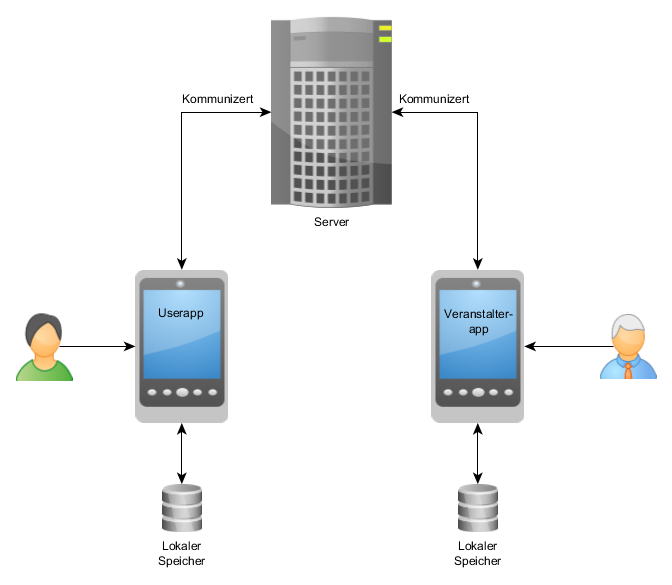
\includegraphics[width=\textwidth]{graphics/Interaktionsmodell.png}
\caption{Ein Interaktionsmodell der User- und Veranstalter-App}
\label{fig:UserAppUndVeranstalterAppInteraktionsmodell}
\end{figure}
Das Projekt umfasst zwei Apps, eine App für die Veranstalter(Veranstalterapp) von Skatenights und eine App für die Teilnehmer(Userapp) von Skatenights. In beiden Apps hat man eine Liste von Veranstaltungen gegeben und man kann einzelne Veranstaltungen aus dieser Liste betrachten. In der Veranstalterapp hält ein Fragment, das \KLASSE{ShowEventsFragment}, die Liste von Veranstaltungen und in der Userapp wird dies mit einer Activity, der \KLASSE{ShowEventsActivity}, realisiert. Die Liste ist ein \KLASSE{ListView} Element, welches in der dazugehörigen xml Datei des Fragments/ der Activity definiert wird, das über einen Adapter gefüllt wird. In beiden Apps wird dazu der gleiche Adapter, der \KLASSE{EventsCursorAdapter}, benutzt. Auf den Adapter wird näher in Abschnitt \ref{sec:adapter} eingegangen. Nach dem Auswählen einer Veranstaltung aus der Liste wird eine Activity gestartet, um die Informationen der Veranstaltung anzuzeigen. In den Informationen einer Veranstaltung kann man sich die Karte über eine neue Activity anschauen. Um auf den Server zuzugreifen benutzen beide Apps sogenannte Tasks. Ein Task ist eine Java Klasse, welche \KLASSE{AsyncTask} erweitert und bei Aufruf einen neuen Thread erstellt um mit dem Server zu kommunizieren. Ein Task hat meist zwei implementierte Methoden, die \METHODE{doInBackground(...)} und die \METHODE{onPostExecute(...)}. Der Server Zugriff erfolgt meist in der \METHODE{doInBackground(...)} Methode, die \METHODE{onPostExecute(...)} Methode wird erst nach kompletten Durchlauf der \METHODE{doInBackground(...)} Methode aufgerufen. Diese Methode wird meistens dazu genutzt um das Ergebnis des Tasks an die Userapp bzw. an die Veranstalterapp zu übergeben. Folgende Tasks werden sowohl in der Userapp als auch in der Veranstalterapp genutzt: 

\KLASSE{GetEventTask}: Dieser Task erwartet die ID einer Veranstaltung und ruft dann die dazu passende Veranstaltung vom Server ab, null falls keine Veranstaltung mit der angegebenen ID existiert. Der Aufruf erfolgt, wenn ein Benutzer eine Veranstaltung in der Liste auswählt um sich die Informationen anzeigen zu lassen.

\KLASSE{QueryEventsTask}: Dieser Task ruft die komplette Liste von Veranstaltungen vom Server ab und gibt diese aus, null falls keine Veranstaltungen auf dem Server existieren. Der Aufruf erfolgt, wenn ein Benutzer die Userapp bzw. die Veranstalterapp startet oder die Liste in der Userapp aktualisiert wird.

\subsection{Beschreibung Veranstalter-App}
\subsubsection{Gerüst}
\AUTHOR{Martin und Bernd}
\begin{figure}[htb]
\centering
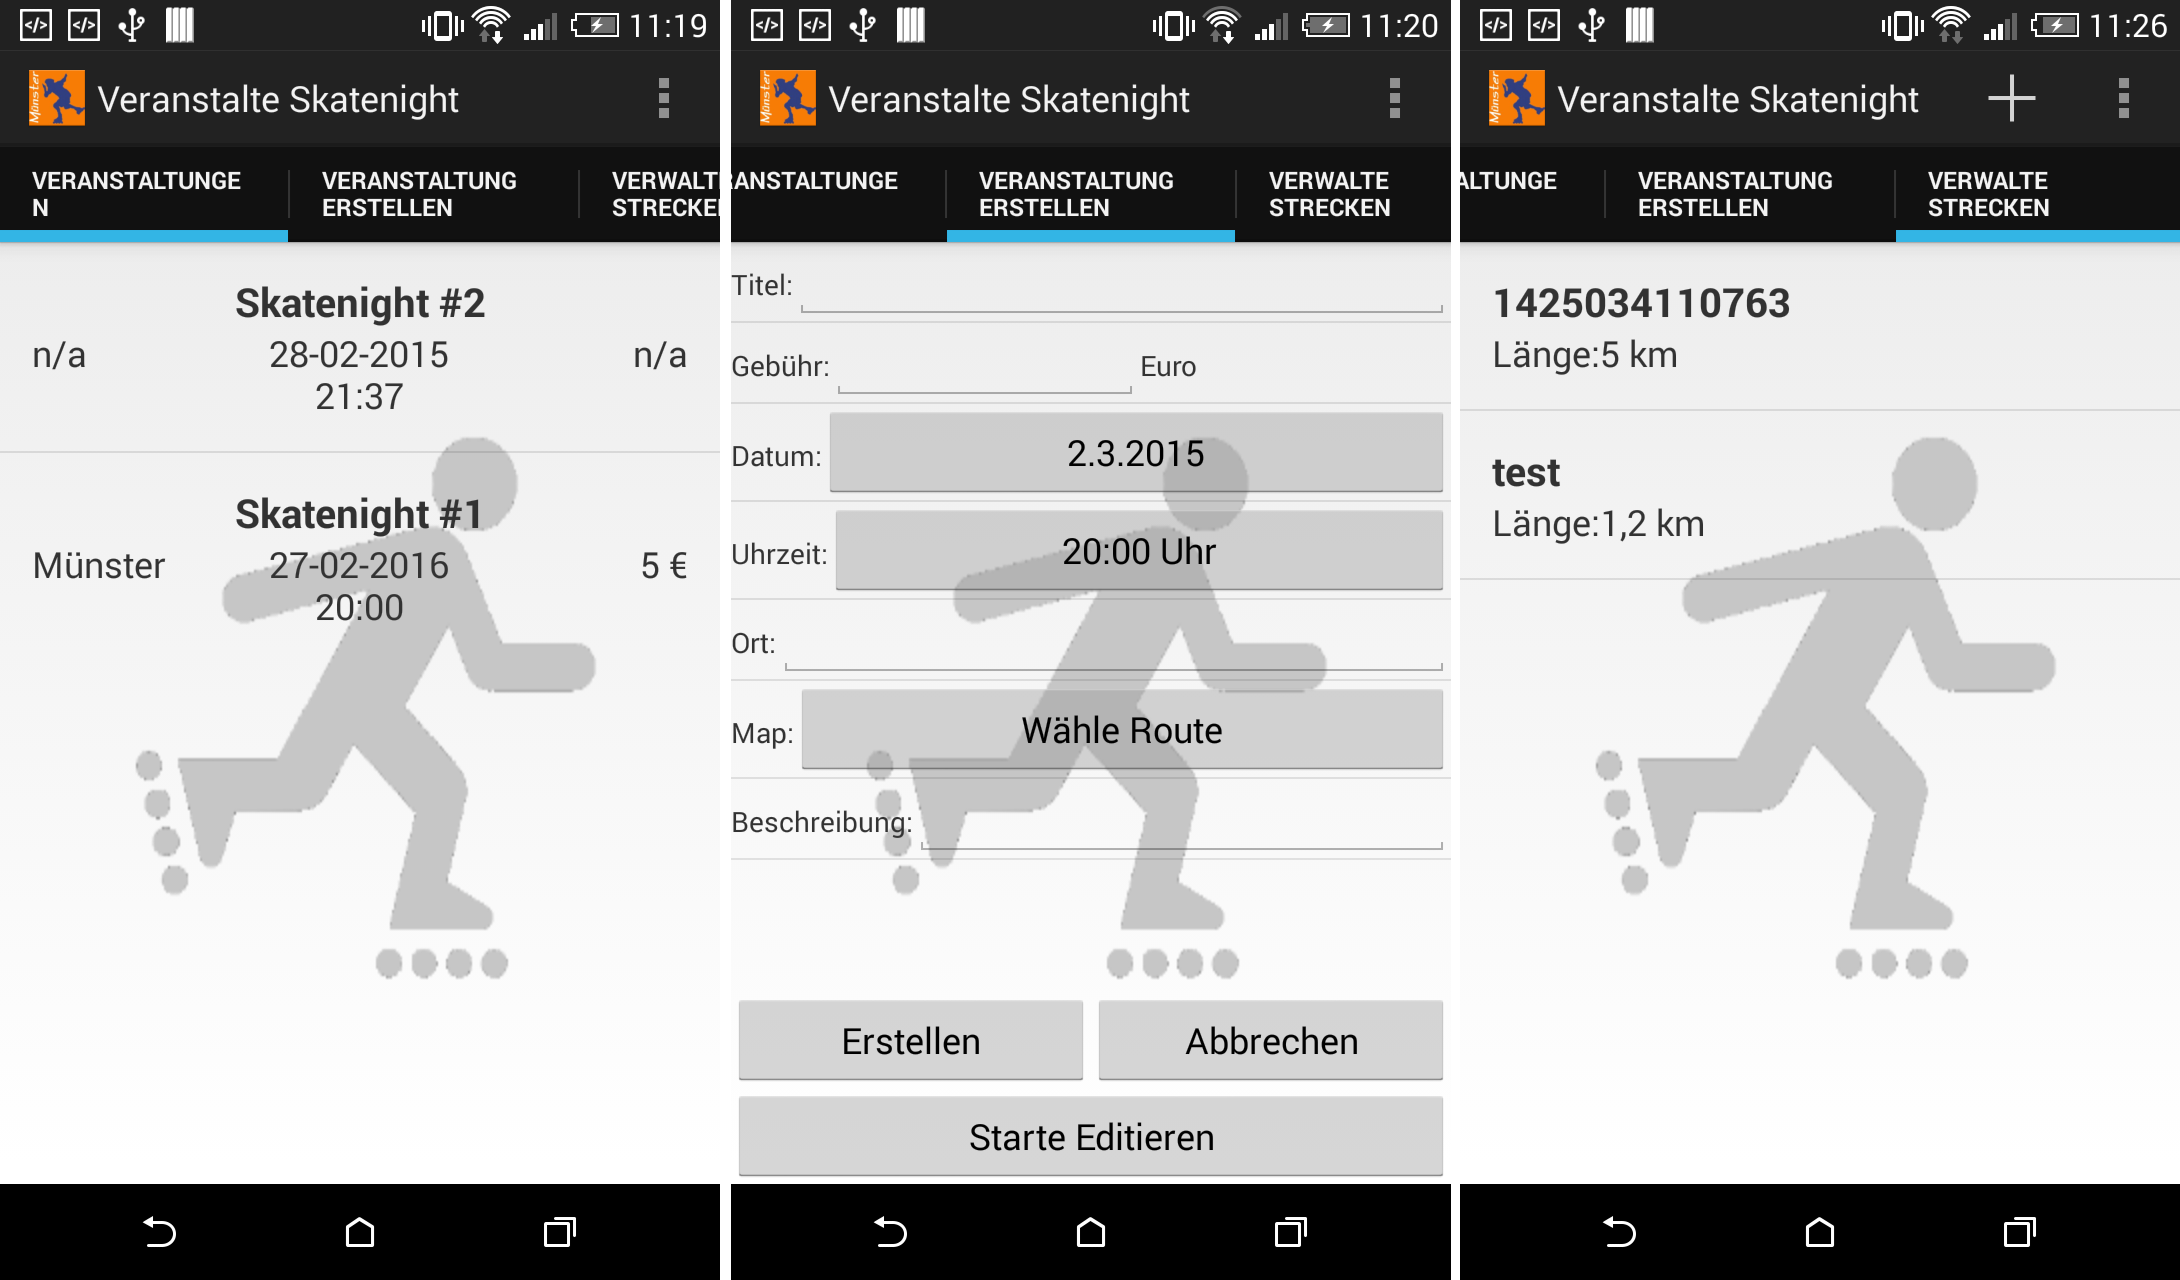
\includegraphics[width=\textwidth]{graphics/veranstalterapp_events.png}
\caption{Eine Übersicht über die in der Veranstalter-App angebotenen Fragments}
\label{fig:veranstalterapp_fragments}
\end{figure}

Um zu den eigentlichen Funktionen der Veranstalterapp zu gelangen muss man sich zu Beginn in der \KLASSE{LoginActivity} mit seinem Google-Account einloggen. Ist der Login erfolgreich, so wird die \KLASSE{HoldTabsActivity} gestartet.

Die Veranstalterapp besteht aus einer Activity, der \KLASSE{HoldTabsActivity}, die einen Viewpager nutzt um zwischen den Funktionalitäten der App zu navigieren. Ein Viewpager ist eine UI-Komponente, welche dafür sorgt, dass man zwischen verschiedenen Tabs über horizontales Scrollen bzw. über Klicken der Tabs in der Tab-Leiste (siehe Abbildung) wechseln kann. Jeder einzelne Tab ist in dem Fall ein einzelnes Fragment. Dazu ist ein Adapter erforderlich, der entscheidet welches Fragment angezeigt werden soll, wenn gescrollt wird, bzw. wenn auf einen der Tabs geklickt wird. Dieser Adapter(\KLASSE{TabsPagerAdapter}) ist eine Klasse, welche \KLASSE{FragmentPagerAdapter} erweitert und zwei Methoden benötigt um Fragmente zu verwalten. Der \KLASSE{TabsPagerAdapter} hält eine Liste der Fragmente die im Konstruktor dieser hinzugefügt werden. Eine der beiden Methoden ist die \METHODE{getItem(...)} Methode. Diese wird aufgerufen, wenn ein Tab berührt wird oder in einem Fragment horizontal gescrollt wird und liefert das Fragment mit dem übergebenen Index in der Liste zurück. Durch die \METHODE{getCount(...)} Methode weiß der Adapter wie viele Tabs höchstens angezeigt werden sollen. Wenn die Activity gestartet wird, dann wird in der \METHODE{onCreate(...)} Methode der ViewPager, der Adapter(\KLASSE{TabsPagerAdapter}) und die Namen der Tabs initialisiert. Anschließend muss dieser Adapter dem ViewPager hinzugefügt werden, damit die Fragmente angezeigt werden können. Es werden insgesamt drei Fragmente dem Adapter hinzugefügt. Das \KLASSE{ShowEventsFragment} dient dem Anzeigen aller Veranstaltungen und ist das Fragment, das beim Start der Veranstalterapp angezeigt wird. In der Liste von Veranstaltungen kann man genauere Informationen einzelner Veranstaltungen durch das Auswählen betrachten, ändern und auch löschen. Das \KLASSE{AnnounceInformationFragment} dient zum Erstellen neuer Veranstaltungen. Man hat hier die Möglichkeit weitere Angaben zu der Veranstaltung hinzuzufügen, als die standardmäßig festgelegten. Dies wird in Abschnitt \ref{sec:events} genauer beschrieben. Das \KLASSE{ManageRoutesFragment} dient zum Verwalten aller auf dem Server vorhandenen Routen. Man hat hier die Möglichkeit Routen hinzuzufügen, zu löschen und als Vorlage für neue Routen zu benutzen. Des weiteren ist nur wenn dieses Fragment angezeigt wird der \glqq Routen hinzufügen\grqq-Button in der ActionBar sichtbar. Dazu erweitert das \KLASSE{ManageRoutesFragment} das OptionsMenu der \KLASSE{HoldTabsActivity} um den zusätzlichen Button in der \METHODE{onCreateOptionsMenu(...)} Methode. Damit dies umgesetzt wird muss beim Erstellen des Fragmentes in der \METHODE{onCreate(...)} Methode mit dem Aufruf \METHODE{setHasOptionsMenu(...)} signalisiert werden, dass eine Erweiterung der ActionBar vorliegt. Die \KLASSE{HoldTabsActivity} bietet die Möglichkeit über das Menu der ActionBar die Rechteverwaltung aufzurufen. 

\FloatBarrier
\subsubsection{Hosts}
\AUTHOR{Bernd}

\begin{figure}[htb]
\centering

\includegraphics[width=6cm]{graphics/Hosts.png}
\caption{Die Liste der eingetragenen Veranstalter}
\label{fig:hosts}
\end{figure}

Ein Host ist ein Veranstalter, welcher autorisiert ist die Veranstalterapp zu starten und die dortigen Funktionen zu nutzen. Ein Host ist eine Klasse auf dem Server, mit einem Attribut Key für den Schlüssel eines Hostobjekts und einem String für die E-Mail. In der Veranstalterapp ist es Hosts erlaubt andere Hosts hinzuzufügen und auch zu löschen. Um dies zu tun muss man die Veanstalterapp starten und dann das Optionsmenü aufrufen. Dort kann man dann \glqq Rechte\grqq\ auswählen und man wird zu der Recheverwaltung weitergeleitet. Die Rechteverwaltung ist lediglich eine Activity(\KLASSE{PermissionManagementActivity}) mit einer ListView für die Liste der Hosts, die zum Zeitpunkt des Aufrufs der Activity auf dem Server existieren. Wenn die Activity gestartet wird, fragt diese in der \METHODE{onCreate(..)} Methode alle Hosts vom Server ab. Dazu wird der \KLASSE{QueryHostsTask} aufgerufen, welcher die Liste vom Server in der \METHODE{doInBackground(...)} Methode abfragt, und diese dann in der \METHODE{onPostExecute(...)} an die Activity weiter gibt, indem der Task die \METHODE{setHostsToListView(...)} in der Activity aufruft. Diese Methode in der Activity erstellt einen neuen Adapter(\KLASSE{HostCursorAdapter}) welcher der ListView hinzugefügt wird.\\
\FloatBarrier

\PARAGRAPH{Hinzufügen und Löschen von Hosts}

\begin{figure}[htb]
\centering
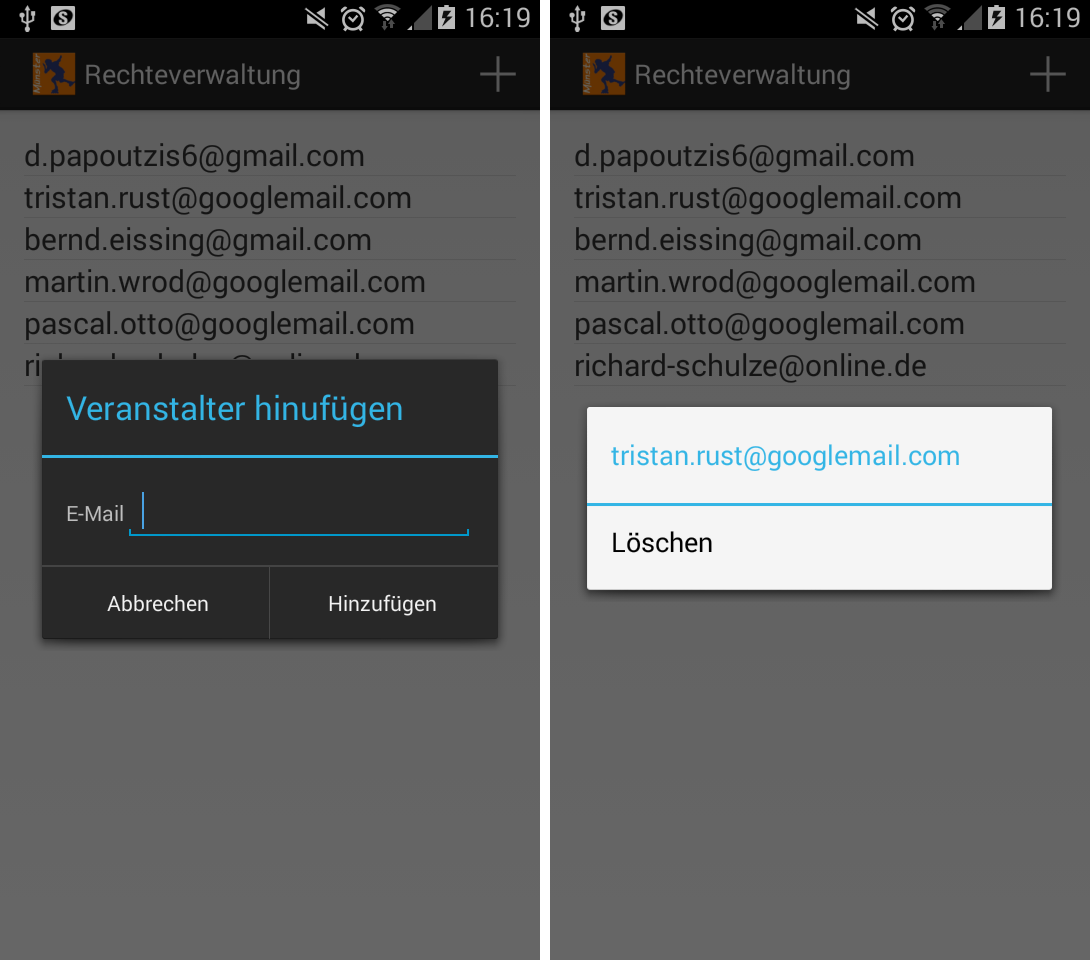
\includegraphics[width=12cm]{graphics/Host_hinzufuegen_loeschen.png}
\caption{GUI zum Hinzufügen und Löschen von Veranstaltern}
\label{fig:hosts_hinzufuegen_Loeschen}
\end{figure}

Es sind Optionen zum Hinzufügen und Löschen von Hosts vorhanden. Zum Löschen eines Hosts muss man im Actionmenu den Plusbutton betätigen. Dadurch wird eine neue Activity(\KLASSE{AddHostDialog}) gestartet, welche einen EditText für die E-Mail des neuen Host und zwei Buttons für das Abbrechen und das Bestätigen des Vorgangs hat. An dieser Stelle wird nicht geprüft, ob es sich bei dem angegebenen Text um eine E-Mail handelt oder nicht; es wird lediglich abgefragt, ob der angegebene Text nicht leer ist. Der Abbrechen-Button beendet den Vorgang. Bei Eingabe und Bestätigung durch Drücken des Hinzufügen Buttons wird die \METHODE{apply(...)} Methode aufgerufen, welche den \KLASSE{AddHostTask} startet. Dieser Task erwartet einen String und ruft dann auf dem Server die \METHODE{addHost(...)} Methode auf. Veranstalter können auch aus der Liste von Veranstalter gelöscht werden. Dazu muss man die gewünschte E-Mail eines Veranstalters in der Liste berühren. Es wird ein AlertDialog gestartet, welcher als Überschrift die E-Mail des ausgewählten Veranstalters hat und einen Löschen Button. Bei Betätigung des Löschen Buttons wird der \KLASSE{DeleteHostTask} aufgerufen, welcher einen String für die E-Mail eines Hosts erwartet und damit dann in der \METHODE{doInBackground(...)} Methode die \METHODE{removeHost(...)} Methode auf dem Server aufruft. In der \METHODE{onPostExecute(...)} Methode wird dann die Liste von Veranstaltern  in der Activity durch den Aufruf von \METHODE{refresh(...)} aktualisiert. Momentan kann jeder Veranstalter alle möglichen Strings als Veranstalter hinzufügen, da nicht geprüft wird ob es sich um den angegebenen Text um eine E-Mail handelt. Des weiteren kann ein Veranstalter sich selber löschen, was dazu führt, dass dieser in der Veranstalterapp keine Funktionen mehr betätigen kann aber dennoch eingeloggt ist.
\FloatBarrier

\subsubsection{Routen}
\AUTHOR{Pascal}
Das Erstellen und Bearbeiten von Routen ist ein integraler Bestandteil der Veranstalter-App. Dem Nutzer sollte es möglich sein auf intuitive Weise Strecken zu erstellen ohne diese selber abzulaufen oder umständlich manuell auf der Karte zu zeichnen. Stattdessen sollte die Strecke möglichst automatisch über die bestehenden Straßen gelegt werden. Da das Erstellen einer Strecke eine einzelne unabhängige Aktivität darstellt, wird mit der \KLASSE{RouteEditorActivity} eine eigene Activity bereitgestellt die sich allein mit dieser Aufgabe beschäftigt. Diese Activity beinhaltet einen ViewPager welcher zwei Fragments verwaltet zwischen denen sowohl über die Tab Leiste, als auch durch horizontales wischen gewechselt werden kann (genauere Beschreibung in Abschnitt \ref{sec:appGeruest}). Verwaltet werden das \KLASSE{EditorMapFragment}, welches die Darstellung und Bearbeitung der Strecke auf der Karte ermöglicht und das \KLASSE{EditorWaypointsFragment}, welches die Bearbeitung einzelner Wegpunkte in der Liste ermöglicht. Die Fragment Klassen beinhalten lediglich die Methoden zur Abstraktion des UI welche von der eigentlichen Programmlogik in der \KLASSE{RouteEditorActivity} aufgerufen werden.

Von der \KLASSE{RouteEditorActivity} verwaltete Daten werden hauptsächlich durch zwei statische innere Klassen repräsentiert. Diese kombinieren die von der \glqq Google Maps Android API v2\grqq\ gestellten Klassen zur Darstellung der Daten auf der Strecke mit zusätzlichen Metainformationen. Um die Verwendung dieser Klassen zu erleichtern implementieren sie das Parcelable Interface. Somit können sie beispielsweise in der \METHODE{onSaveInstanceState(Bundle)} problemlos im Bundle hinterlegt werden. Referenzen auf UI Elemente werden jedoch nicht gespeichert (siehe Abschnitt \ref{par:GoogleMapsAndroidAPI}). Die erste dieser Klassen ist die \KLASSE{RouteEditorActivity.Route}, welche den Streckenverlauf der berechneten Route darstellt. Sie kombiniert die von Google Maps genutzten \KLASSE{PolylineOptions} und \KLASSE{Polyline} mit der als int gespeicherten Länge der Strecke in Metern. Die zweite der Klassen ist die \KLASSE{RouteEditorActivity.Waypoint}, welche einen einzelnen Wegpunkt auf der Strecke darstellt. Diese bestehen aus den von Google Maps genutzten \KLASSE{MarkerOptions} und \KLASSE{Marker}.

\PARAGRAPH{Google Maps Android API v2}
\label{par:GoogleMapsAndroidAPI}
Die Google Maps Android API v2 ist Teil der Google Play Services und bietet die Möglichkeit einfach zu verwendende, interaktive Karten in Android Apps zu verwenden. Kernstück der API ist die \KLASSE{GoogleMap} Klasse, welche Interaktion mit der dargestellten Karte ermöglicht. Zugriff erfolgt wahlweise über die \METHODE{getMap()} Methoden der \KLASSE{MapView} oder \KLASSE{MapFragment} Klassen, welche zur Darstellung der Karte verwendet werden. Da die Karte Zugriff auf den Activity-Lifecycle benötigt, wird von Google die Verwendung des \KLASSE{MapFragment} empfohlen. Die \KLASSE{GoogleMap} stellt eine Vielzahl von Möglichkeiten bereit die Karte der erforderten Nutzung anzupassen. Insgesamt werden 6 mögliche Varianten für Kartenannotationen bereitgestellt: Circle, GroundOverlay, Marker, Polygon, Polyline und TileOverlay. Für die Planung der Route benötigen wir jedoch lediglich \KLASSE{Marker} für die Darstellung von Wegpunkten und eine \KLASSE{Polyline} für die Darstellung des Streckenverlaufs. Diese Annotationen bestehen jeweils aus zwei Teilen. So repräsentiert die \KLASSE{MarkerOptions} Klasse Anweisungen um einen \KLASSE{Marker} auf der Karte darstellen zu können. Um diesen tatsächlich darzustellen wird die \METHODE{addMarker(MarkerOptions)} Methode der \KLASSE{GoogleMap} aufgerufen. Diese liefert eine Referenz auf das gezeichnete \KLASSE{Marker} Objekt zurück. Da die \KLASSE{MarkerOptions} lediglich die Anweisungen zum Zeichnen des Markers repräsentieren, müssen Änderungen wie z.B. ein neuer Titel an das \KLASSE{Marker} Objekt übermittelt werden. Da die \METHODE{addMarker(MarkerOptions)} die einzige Möglichkeit darstellt auf dieses zuzugreifen, ist es wichtig das Objekt für eine mögliche spätere Verwendung zu behalten. Zudem muss bedacht werden, dass die \KLASSE{Marker} nur zeitlich begrenzt gültig sind. Wird z.B. durch drehen des Gerätes das UI neu gezeichnet, werden die Marker ungültig. Für diesen Fall sollten die \KLASSE{MarkerOptions} gespeichert werden um die erneute Darstellung zu ermöglichen. Dieses Konzept überträgt sich auf die anderen Annotationstypen z.B. mit \KLASSE{PolygonOptions} und \KLASSE{Polygon}, \KLASSE{PolylineOptions} und \KLASSE{Polyline}, usw. Diese bieten jeweils eigene Schnittstellen um sie auf die Bedürfnisse der Anwendung anzupassen.

Ein Marker besteht aus einem Bild, welches auf der Karte angezeigt wird. Bei Berührung des Bildes wird der Titel des Markers angezeigt. Die Position des Bildes kann mithilfe eines \KLASSE{LatLng} Objektes gesetzt werden, welches aus jeweils einem double Wert für Längen- und Breitengrad besteht. Marker können zudem, falls dies erfordert wird, vom Nutzer nachträglich per drag-and-drop verschoben werden. Die Funktionalität wird über ein einzelnes Flag gesteuert, auf welches man mithilfe der \METHODE{draggable(boolean)} Methode des \KLASSE{Marker} bzw. \KLASSE{MarkerOptions} Objektes zugreifen kann. Auf die neue Position kann über die \METHODE{getPosition()} Methode zugegriffen werden. Zudem besteht die Möglichkeit vom \KLASSE{GoogleMap} Objekt über Veränderungen der Marker durch den Nutzer benachrichtigt zu werden. Dies wird mithilfe des \KLASSE{GoogleMap.OnMarkerDragListener} Interfaces realisiert, welches beim \KLASSE{GoogleMap} Objekt über die \METHODE{setOnMarkerDragListener(GoogleMap.OnMarkerDragListener)} Methode registriert werden kann. Bei Änderungen eines Markers werden danach die \METHODE{onMarkerDragStart(Marker)}, \METHODE{onMarkerDrag(Marker)} und \METHODE{onMarkerDragEnd(Marker)} Methoden aufgerufen.
	
Eine \KLASSE{Polyline} stellt eine Linie dar die auf der Karte gezeichnet wird. Sie besteht hauptsächlich aus einer Farbe, welche die Farbe der Linie kontrolliert und einem float Wert, der die Breite der Linie kontrolliert. Der Verlauf der Linie kann mithilfe der \METHODE{addAll(List<LatLng>)} Methode festgelegt werden. Zugriff auf diese Liste ist über die \METHODE{getPoints()} Methode möglich.

\PARAGRAPHOPT{Google Directions API}{Google Directions API\footnote{https://developers.google.com/maps/documentation/directions/}}
\label{par:GoogleDirectionsAPI}
Über die Google Directions API stellt Google die in Google Maps integrierte Funktionalität zur Planung von Routen zur Verfügung. Per HTTP-Anfrage kann die benötigte Route wahlweise im XML oder JSON Format angefordert werden. Android verfügt bereits über die Funktionalität zum parsen von XML und JSON, sodass wir uns nach der Empfehlung von Google richten und das JSON Format verwenden. In der kostenlosen Variante sind die Anzahl der Anfragen auf 2500 pro Tag limitiert. Da die API jedoch ausschließlich beim Eintragen der Route durch die Veranstalter genutzt wird, kann dies vernachlässigt werden. API Anfragen richten sich an \glqq http://maps.googleapis.com/maps/api/directions/\grqq\ gefolgt von dem gewünschten Ausgabeformat. In diesem Fall folgt also \glqq.../directions/json?\grqq. Anschließend können eine Reihe von Parametern in beliebiger Reihenfolge übergeben werden, die durch \glqq\&\grqq\ getrennt werden. Zunächst gibt es jeweils einen Parameter für Ausgangs- und Zielpunkt. Diese können als \glqq origin=\grqq\ und \glqq destination=\grqq\ gefolgt von den gewünschten Adressen übergeben werden. Adressen werden automatisch zu Koordinaten umgewandelt. Alternativ können die Koordinaten auch direkt als Längen- und Breitengrad getrennt durch ein \glqq,\grqq\ übergeben werden. Um den Routenverlauf genauer zu Steuern, können zusätzlich Wegpunkte übermittelt werden. Dies erfolgt mithilfe des \glqq waypoints=\grqq\ Parameters gefolgt von einer Reihe von Adressen, die das gleiche Format wie Start- und Endpunkt unterstützen. Die einzelnen Adressen werden durch ein \glqq|\grqq\ getrennt. Übergebene Wegpunkte werden in der angegebenen Reihenfolge in die Route integriert. An dieser Stelle fällt bei der kostenlosen Variante der API eine weitere Einschränkung an. So dürfen neben dem Start und Endpunkt maximal 8 Wegpunkte angegeben werden. Zuletzt gibt es noch den \glqq sensor=\grqq\ Paramter welcher der API über einen Boolean Wert mitteilt ob das Gerät über die Möglichkeit verfügt seinen Standort zu ermitteln. Eine einfache Route an der Straße um das Hörsaalgebäude an der Einsteinstraße über zwei Wegpunkte lässt sich somit über die folgende Anfrage planen:

http://maps.googleapis.com/maps/api/directions/json?origin=51.965516,7.603414

\&destination=51.965674,7.604188\&waypoints=51.968710,7.603574|51.967477,7.606374

\&sensor=true

Der zurückgegebene JSON String enthält ein Objekt \glqq status\grqq, welches den Statuscode der Anfrage enthält, und ein Array \glqq routes\grqq, welches die gefundenen Routen enthält. Konnte keine Route gefunden werden, ist \glqq routes\grqq\ leer und Status enthält den Grund für den Fehler. Die genauen Fehlercodes finden sich in der Dokumentation unter \glqq Statuscodes\grqq. Gefundene Routen bestehen aus einer Anzahl von Metainformationen und einer detaillierten Beschreibung der Route. Da für die Anwendung lediglich der Streckenverlauf relevant ist, können die meisten dieser Informationen ignoriert werden. Die Beschreibung der Route ist unterteilt in mehrere Streckenabschnitte, die sich im \glqq legs\grqq\ Array der Route befinden. Diese Streckenabschnitte enthalten neben einer Zusammenfassung des Abschnittes die genauen Anweisungen im \glqq steps\grqq\ Array. Jede Anweisung besteht unter anderem aus dem genauen Straßenverlauf (\glqq polyline.points\grqq), Informationen über den Abschnitt (z.B. \glqq distance.value\grqq) und einer textuellen Fahranweisung (\glqq html\_instructions\grqq).

\PARAGRAPH{RouteEditorActivity Funktionalität}
Die \KLASSE{RouteEditorActivity} ist die Zentrale Klasse des Interface zum Erstellen von Routen. Beim starten der Activity wird der Name der Route als String Extra (\ATTRIBUT{RouteEditorActivity.EXTRA\_NAME}) erwartet. Dieser wird im Member \ATTRIBUT{name} gespeichert. Mithilfe des \ATTRIBUT{RouteEditorActivity.EXTRA\_WAYPOINTS} können außerdem Wegpunkte als Ausgangspunkt für die Strecke übergeben werden. Zur Verwaltung der Wegpunkte wird mit dem \KLASSE{WaypointAdapter} ein modifizierter ArrayAdapter verwendet, welcher angepasst wurde um die Namen der Wegpunkte aus den \KLASSE{MarkerOptions} des \KLASSE{Waypoint} zu lesen. Das \KLASSE{Route} Objekt, welches die aktuell berechnete Strecke repräsentiert wird im Member \ATTRIBUT{route} hinterlegt. Falls keine Route vorhanden ist, nimmt dieses den Wert null an. Damit beim Drehen des Bildschirms keine Berechnungen verloren gehen, werden Name, Route und Wegpunkte im Bundle gespeichert. Da die \KLASSE{Route} und \KLASSE{Waypoint} Klassen das Parcelable Interface implementieren, können diese im Bundle mithilfe der \METHODE{putParcelable(String, Parcelable)} bzw. \METHODE{putParcelableArray(String, Parcelable[])} gespeichert werden. Um eine Strecke zu erstellen müssen zunächst mindestens zwei Wegpunkte hinzugefügt werden. Das Erstellen neuer Wegpunkte geschieht mithilfe der \METHODE{addWaypoint()} Methode. Diese kann von beliebiger Stelle aufgerufen werden. In der App geschieht dies ausschließlich über einen Button in der ActionBar. Der neue \KLASSE{Waypoint} wird mithilfe der \METHODE{addWaypoint(int)} Methode des \KLASSE{EditorMapFragment} erstellt, welche den Mittelpunkt der Karte ermittelt und diesen als Position des Waypoints übernimmt. Außerdem wird der Titel des \KLASSE{Waypoint} gemäß des übergebenen Index auf \glqq Wegpunkt X\grqq\ gesetzt. Mithilfe des \KLASSE{MarkerOptions} Objektes des \KLASSE{Waypoint} kann der Wegpunkt nun der Karte hinzugefügt werden. Die Referenz für das entstehende \KLASSE{Marker} Objekt wird im \KLASSE{Waypoint} gespeichert. Anschließend versucht die \KLASSE{RouteEditorActivity} die Strecke durch den Aufruf der \METHODE{loadRoute()} Methode zu berechnen. Diese entfernt zunächst mithilfe der \METHODE{setRoute(Route)} Methode die aktuell angezeigte Strecke von der Karte und berechnet anschließend mithilfe des \KLASSE{RouteLoaderTask} eine aktuelle Route, wenn nach der Änderung mindestens zwei Wegpunkte vorhanden sind. Damit der Nutzer weiß, dass die Route berechnet wird, wird in der ActionBar eine auf \ATTRIBUT{indeterminate} gesetzte ProgressBar angezeigt. Beim Beenden des Task, sei es durch Erfolg oder Fehler, wird diese ausgeblendet und die neue Strecke bzw. eine Fehlermeldung angezeigt. Erfolgt ein weiterer Aufruf der Methode, bevor der Task beendet wird, so wird nicht auf dessen Ende gewartet. Stattdessen wird sein Ergebnis ignoriert und auf das Ergebnis des neuen Tasks gewartet. Im Member \ATTRIBUT{currentTask} wird dafür eine Referenz auf den Task behalten, dessen Ergebnis dem zeitlich neuesten Aufruf der \METHODE{loadRoute()} Methode entspricht. 

Da die Wegpunkte im \KLASSE{WaypointAdapter} gespeichert werden, spiegeln sich Änderungen direkt in der ListView im \KLASSE{EditorWaypointsFragment} wieder.
	
Das Fragment behandelt insgesamt nur zwei Funktionalitäten. Zum einen wird ein \KLASSE{AdapterView.OnItemClickListener} verwendet, welcher beim Berühren eines Wegpunktes in der Liste das \KLASSE{EditorMapFragment} im ViewPager aktiviert und mithilfe dessen \METHODE{showWaypoint(Waypoint)} Methode den Wegpunkt auf der Karte vergrößert und dessen Titel anzeigt. Außerdem wird ein \KLASSE{AdapterView.OnItemLongClickListener} verwendet, welcher bei seiner Aktivierung durch ein langes drücken auf einen der Wegpunkte in der Liste die Option zum Benennen und Löschen dieses Wegpunktes anzeigt.  Beim Löschen wird die \METHODE{removeWaypoint(int)} Methode der \KLASSE{RouteEditorActivity} aufgerufen welche den Wegpunkt aus dem Adapter entfernt, ihn beim \KLASSE{EditorMapFragment} mithilfe der \METHODE{removeWaypoint(Waypoint)} von der Karte entfernt, die Indizes der folgenden Wegpunkte aktualisiert und mithilfe der \METHODE{loadRoute()} falls möglich eine neue Route berechnet.

Auch das \KLASSE{EditorMapFragment} bietet eine Möglichkeit den Streckenverlauf zu ändern. So implementiert dieses das \KLASSE{GoogleMap.OnMarkerDragListener} Interface, welches von der \KLASSE{GoogleMap} über das Verschieben eines der Marker benachrichtigt wird. Wir müssen lediglich auf den Aufruf der \METHODE{onMarkerDragEnd(Marker)} Methode warten, um den \KLASSE{Waypoint} über die Positionsänderung zu benachrichtigen. Da beim Verschieben des Marker lediglich die Position des Marker beeinflusst wird, muss diese Änderung auf das \KLASSE{PolylineOptions} Objekt übertragen werden. Anschließend wird noch die \METHODE{loadRoute()} Methode der \KLASSE{RouteEditorActivity} aufgerufen damit diese die geänderte Route berechnen kann.

\PARAGRAPH{RouteLoaderTask Funktionalität}
Der \KLASSE{RouteLoaderTask} ist für die eigentliche Routenberechnung verantwortlich. Er interagiert dafür mithilfe von HTTP-Anfragen mit der Google Directions API. Da es sich bei diesen Interaktionen um Netzwerkanfragen handelt, die möglicherweise längere Ladezeiten mit sich bringen, dürfen diese nicht auf dem UI-Thread ausgeführt werden, damit dieser nicht unnötig blockiert wird. Das Android SDK stellt hier in Form des \KLASSE{AsyncTask} eine nützliche Klasse bereit, welche eine zusammenhängende Berechnung auf einem Hintergrund-Thread repräsentiert. In seiner ursprünglichen Form bietet der \KLASSE{AsyncTask} mithilfe der \METHODE{onProgress(Progress)} und \METHODE{onPostExecute(Result)} Methoden die Interaktion mit dem GUI. In der \DATEI{common} Bibliothek findet sich mit dem \KLASSE{ExtendedTask} eine Unterklasse des \KLASSE{AsyncTask}, welcher um die Funktionalität erweitert wurde den Fortschritt, das Ergebnis und mögliche Fehlermeldungen direkt an ein \KLASSE{ExtendedTaskDelegate} zu übertragen. Die \KLASSE{RouteEditorActivity} implementiert dieses Interface zu diesem Zweck. 

In der \METHODE{doInBackground(ArrayAdapter<Waypoint>...)} Methode findet die Routenberechnung und die anschließende Auswertung statt. Diese wird im Hintergrund-Thread des \KLASSE{ExtendedTask} ausgeführt. Mithilfe der \METHODE{publishProgress(Progress)} und \METHODE{publishError(String)} Methoden kann mit der \KLASSE{ExtendedTaskDelegate} interagiert werden. Dabei ist zu beachten, dass nach einem Aufruf der \METHODE{publishError(String)} Methode ein eventuell übergebenes Ergebnis nicht an die Delegate weitergeleitet wird. Die erste Aufgabe des Task ist die Erstellung der HTTP-Anfrage, nach dem in Kapitel \ref{par:GoogleDirectionsAPI} beschriebenen Schema. Dafür wird der von Android bereitgestellte \KLASSE{Uri.Builder} verwendet. Dieser kann von einer Base-URL ausgehend Parameter automatisch korrekt formatieren. Es werden dafür lediglich der Name des Parameters und der zugehörige Wert als String benötigt. In diesem Fall werden automatisch der erste Wegpunkt des übergebenen ArrayAdapter als \glqq origin\grqq\ und der letzte als \glqq destination\grqq\ verwendet. Für die Umwandlung von \KLASSE{LatLng} zu String steht die \METHODE{positionToString(LatLng)} Methode zur Verfügung. Sie wandelt Längen- und Breitengrad von double Werten in Strings um und kombiniert diese, getrennt durch ein \glqq,\grqq\ zu einem einzelnen String. Die \METHODE{waypointsToString(ArrayAdapter<Waypoint>)} Methode kombiniert mithilfe der \METHODE{positionToString(LatLng)} Methode die enthaltenen Wegpunkte zu einem String, indem sie diese mit dem Trennzeichen \glqq|\grqq\ kombiniert. Da es sich beim 1. und letzten Wegpunkt um den Start- und Endpunkt handelt, werden diese nicht berücksichtigt. Der resultierende String wird im \KLASSE{Uri.Builder} für den Parameter \glqq waypoints\grqq\ eingetragen. Zuletzt wird durch \glqq sensor=true\grqq\ signalisiert, dass das Gerät über einen Standortsensor verfügt. Mit der entstandenen Uri kann nun ein URL Objekt erstellt werden, welches über die \METHODE{openConnection()} Methode eine HTTP Verbindung öffnet. An diese Verbindung wird nun eine \glqq GET\grqq\ Anfrage geschickt. Als Antwort erhalten wir das Ergebnis der geforderten Routenberechnung formatiert als JSON-String. Dieser kann mithilfe der \METHODE{parseJSONString(String)} Methode geparst werden. Als Ergebnis erhalten wir ein Route Objekt mit dem berechneten Streckenverlauf. Die Methode legt zunächst ein JSONObject mit dem empfangenen String an, welches Teil des Android SDK ist. Dieses Objekt stellt unter anderem zwei Methoden zur Verfügung, die entsprechend der Objekthierarchie Zugriff auf unterliegende JSON Objekte bzw. Arrays bietet. Mit der \METHODE{getJSONArray(String)} Methode erhalten wir das JSONArray, welches die einzelnen Routen beinhaltet. Hier reicht es aus die erste enthaltene Route zu verwenden. Die Route enthält in \glqq overview\_polyline.points\grqq\ eine als String codierte Linie, welche den gesamten Routenverlauf umfasst. Diese Linien werden mithilfe des Polyline Algorithmus codiert, welcher es ermöglicht diese kompakt zu speichern. Der Algorithmus ist in der Google Maps Dokumentation\footnote{https://developers.google.com/maps/documentation/utilities/polylinealgorithm} genauer beschrieben; Die Implementation in der \KLASSE{LocationUtils} liefert zudem eine genaue Beschreibung der Funktion. Bei kurzen Strecken entspricht diese Übersichtsstrecke dem tatsächlichen Streckenverlauf, bei längeren Strecken ist dies jedoch nicht garantiert. Aus diesem Grund decodieren wir stattdessen die Strecken der einzelnen Routenanweisungen. Die Anweisungen befinden sich als Array \glqq steps\grqq\ in den Streckenabschnitten, die als Array \glqq legs\grqq\ vorhanden sind. Um also den gesamten Routenverlauf zu erhalten wird im JSONObject welches die Route repräsentiert jedes \glqq legs[i].steps[j].polyline.points\grqq\ decodiert und einer Liste mit \KLASSE{LatLng} Objekten hinzugefügt. Diese wird anschließend dem \KLASSE{PolylineOptions} Objekt des Route Objekts hinzugefügt. Um die Gesamtlänge der Strecke zu erhalten wird dabei auch die im \glqq legs[i].steps[j].distance.value\grqq\ enthaltene Strecke in Metern aufaddiert. Das entstehende Route Objekt wird der \KLASSE{RouteEditorActivity} anschließend als Ergebnis übermittelt.

\PARAGRAPH{Routen als Vorlage nutzen und das Benennen von Wegpunkten}
\AUTHOR{Bernd}

\begin{figure}[htb]
\centering
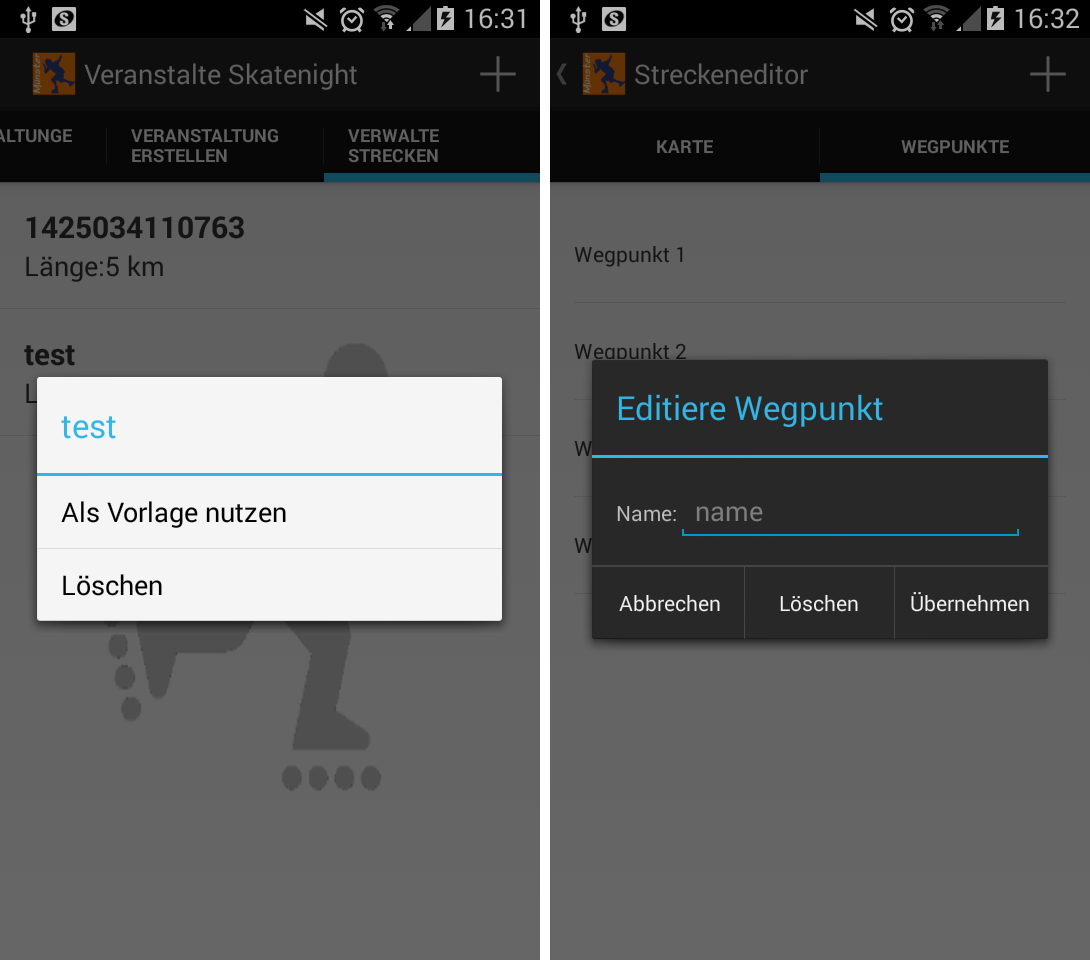
\includegraphics[width=12cm]{graphics/Route_als_Vorlage_nutzen_Wegpunkte_benennen.png}
\caption{Erstellen einer Route aus einer Vorlage und das Umbenennen von Wegpunkten}
\label{fig:route_aus_vorlage}
\end{figure}

Man kann bestehende Routen benutzen um aus diesen neue Routen zu erstellen. Dazu muss man im \KLASSE{ManageRoutesFragment} eine  Route aus der Liste auswählen und einen Longclick darauf machen. Es erscheint ein AlertDialog dessen Überschrift den Namen der Route darstellt. Man hat nun als Auswahl die Route zu löschen oder diese als Vorlage zu nutzen. Wählt man letzteres, so wird die Activity \KLASSE{AddRouteDraftDialog} gestartet. Des weiteren werden als Extras dem Intent die Waypoints der ausgewählten Route beigefügt. Ein Waypoint einer Route ist eine Klasse auf dem Server mit dem Namen \KLASSE{ServerWaypoint}. Ein \KLASSE{ServerWaypoint} hat die Attribute für den Titel eines Waypoints und dessen Latitude und Longitude. Eine Route hat eine Liste von \KLASSE{ServerWaypoints} und diese werden der Route hinzugefügt, wenn die Route erstellt wird, das heißt wenn der AlertDialog zum Speichern einer Route aufgerufen wird. Dort wird dann der \KLASSE{ArrayAdapter} durchlaufen und für jeden Waypoint wird ein \KLASSE{ServerWaypoint} erstellt. Dem ServerWaypoint werden dann der Titel, die Longitude und die Latitude gesetzt und er wird der Liste von ServerWaypoints hinzugefügt. Der Dialog ist eine Activity, in der man ein Feld für den Namen der Route zusammen mit zwei Buttons zum Abbrechen und Bestätigen der Aktion. Gibt man einen Namen für die neue Route ein und bestätigt dies, so wird in der Activity ein Intent gestartet und ihm in den Extras die Waypoints der Route übergeben. Dann wird die \KLASSE{RouteEditorActivity} mit diesem Intent gestartet. In der \METHODE{onCreate(...)} Methode von der \KLASSE{RouteEditorActivitiy} wird dann abgefragt, ob der Intent Extras besitzt und auch, ob dies Waypoints sind. Ist dies der Fall, so  werden die übergebenen Waypoints aus den Extras in ein Attribut gespeichert. Für jeden Waypoint wird dann ein neuer Waypoint erstellt und diesem dann die Latitude,  die Longitude und der Titel gesetzt. Der neue Waypoint wird dann auch noch dem WaypointAdapter hinzugefügt. Der WaypointAdapter erweitert den ArrayAdapter mit dem generischen Typ Waypoint und überschreibt die \METHODE{getView(...)} Methode, sodass für jeden Waypoint eine custom xml Datei angezeigt wird. In dieser Datei bedindet sich eine TextView zum Anzeigen des Namens des Wayoints und dieser wird für jeden Waypoint gesetzt.
\FloatBarrier

\subsubsection{Events}
\label{sec:events}
\AUTHOR{Martin}
Dieser Abschnitt beschäftigt sich mit der Realisierung der Veranstaltungen in der Veranstalter-App. Veranstaltungen können nur von eingetragenen Veranstaltern in der Veranstalter-App erstellt und verwaltet werden und können nach der Erstellung von den Benutzern in der User-App und von allen Veranstaltern in der Veranstalter-App betrachtet werden. Dazu werden die erstellten Veranstaltungen persistent auf dem Server abgespeichert. Zu Beginn des Projekts hatte eine Veranstaltung noch eine feste Anzahl an Informationen, d.h. die Model-Klasse \glqq Event\grqq, die eine Veranstaltung beschreibt, hatte Attribute für den Titel, für die Gebühr, für die Beschreibung usw. Durch Einführung der Features \glqq Veröffentlichen von Informationen 2.0\grqq\ und \glqq Anzeigen von Informationen 2.0\grqq\ musste die Umsetzung überarbeitet werden, da die Anzahl der Informationen zu einer Veranstaltung variabel wurde. Die Realisierung erfolgte nun über dynamische Felder, die eine abstrakte Darstellung einer Information einer Veranstaltung ist. Diese Umsetzung wird im Folgenden behandelt.

\PARAGRAPH{Model-Klasse Event}
Die Klasse Event in unserem Projekt stellt eine Veranstaltung dar. Ein Objekt dieser Klasse beinhaltet alle Informationen einer Veranstaltung.

\begin{figure}[htb]
\centering
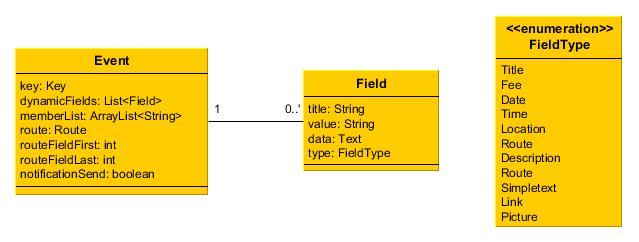
\includegraphics[width=\textwidth]{graphics/Model_Klassen.png}
\caption{Die verwendeten Klassen zur Repräsentation von Veranstaltungen}
\label{fig:modelEvents}
\end{figure}

Zu Beginn werde ich auf die dynamischen Felder und auf die Arten der dynamischen Felder eingehen, die durch die Klassen \KLASSE{Field} und \KLASSE{FieldType} realisiert wurden.\\

\textbf{Klasse Field:}

Ein Objekt der Klasse \KLASSE{Field} stellt ein dynamisches Feld dar. Ein dynamisches Feld wird genutzt um eine Veranstaltung zu beschreiben. Jedes dynamische Feld stellt genau eine Information zu einer Veranstaltung dar und besteht aus:

\begin{itemize}
	\item title: Bezeichnung der Information (z.B. \glqq Titel\grqq, \glqq Gebühr\grqq)
	\item value: Wert der Informationen in Form einer Zeichenkette
	\item data: Feld, das nur für die Speicherung einer Routeninformation genutzt wird, leer bei jeder anderen Information
	\item type: Art des Feldes, ein Enum-Objekt des Enums \KLASSE{FieldTypes}
\end{itemize}

\textbf{Enum FieldType:}

Es existieren zehn verschiedene Arten von dynamischen Feldern, die durch das Enum \KLASSE{FieldType} identifiziert werden können. Folgende Arten von dynamischen Feldern existieren:

\begin{itemize}
	\item Title: Titel
	\item Fee: Gebühr
	\item Date: Datum des Startzeitpunkts
	\item Time: Uhrzeit des Startzeitpunkts
	\item Location: Standort des Startpunkts
	\item Description: Beschreibung
	\item Route: Route, die in der Veranstaltung abgefahren wird
	\item Simpletext: Ergänzende Text-Information
	\item Link: Verweis auf Webseite
	\item Picture: Bild
\end{itemize}

\textbf{Klasse Event:}

Ein Event-Objekt beinhaltet alle Information zu einer Veranstaltung. Folgende Informationen ergeben sich:

\begin{itemize}
	\item key: Eindeutige Nummer, die eine Veranstaltung identifiziert
	\item dynamicFields: Liste von dynamischen Feldern
	\item memberList: Liste von E-Mail Adressen der Teilnehmer
	\item routeFieldFirst: erster Wegpunkt des Feldes(siehe Abschnitt \ref{subsec:Feldberechnung})
	\item routeFieldLast: letzter Wegpunkt des Feldes(siehe Abschnitt \ref{subsec:Feldberechnung})
	\item notificationSend: identifiziert, ob die GCM-Nachricht für das Starten einer Veranstaltung gesendet wurde
\end{itemize}

Wird ein neues Event auf dem Server erstellt, wird automatisch eine Key-ID generiert sodass wir uns nicht um die Generierung einer ID kümmern müssen. Da wir eine variable Anzahl an dynamischen Feldern abspeichern wollen, haben wir uns dazu entschieden, die dynamischen Felder in einer Liste abzuspeichern. Jedes dynamische Feld hat einen eigenen Typen, wobei sich die Typen \glqq Simpletext\grqq, \glqq Link\grqq\ und \glqq Picture\grqq\ von den restlichen Typen unterscheiden, da ein Objekt mit diesen Typen mehrmals in der Liste auftreten können. Die restlichen Typen sind einzigartig und treten nur ein einziges Mal in der Liste auf. Die beiden Felder \ATTRIBUT{routeFieldFirst} und \ATTRIBUT{routeFieldLast} werden für die Feldberechnung genutzt, um den Start und  das Ende des Feldes zu speichern
(siehe Abschnitt \ref{subsec:Feldberechnung}). Das letzte Attribut \ATTRIBUT{notificationSend} speichert ob jemals schon eine Notification, die den Start der Veranstaltung ankündigt, gesendet wurde.\\

\textbf{EventUtils:}

Um den Zugriff und die Verwaltung der dynamischen Felder einer Veranstaltung zu vereinfachen haben wir uns dazu entschieden eine Singleton-Klasse \KLASSE{EventUtils} zu erstellen.

\begin{figure}[htb]
\centering
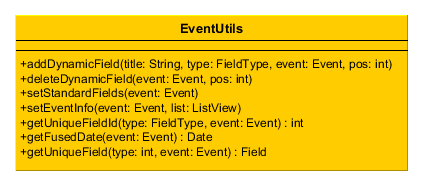
\includegraphics[width=\textwidth]{graphics/EventUtils_long.png}
\label{fig:eventutils}
\end{figure}

Folgende Funktionen bietet die Klasse \KLASSE{EventUtils} an:

\begin{itemize}
	\item addDynamicField: Fügt ein dynamisches Feld mit dem übergebenen Titel und Typ dem Event an der Position \glqq pos\grqq\ hinzu.
	\item deleteDynamicField: Löscht ein dynamisches Feld an der Position \glqq pos\grqq\ aus dem Event.
	\item setStandardFields: Setzt die dynamischen Felder die zu Beginn der Erstellung initialisiert werden sollen(Titel, Gebühr, Startdatum, Startuhrzeit, Ort, Beschreibung, Route).
	\item setEventInfo: Setzt die dynamischen Felder der übergebenen ListView in das übergebene Event-Objekt.
	\item getUniqueFieldId: Gibt die Position des eindeutigen dynamischen Feldes mit dem FieldType \glqq type\grqq\ in der Liste der dynamischen Felder des übergebenen Events zurück.
	\item getFusedDate: Bestimmt aus Startdatum und Startuhrzeit das Datum des Starts mit der Uhrzeit.
	\item getUniqueField: Gibt das einzigartige dynamisches Feld mit dem \KLASSE{FieldType} \glqq type\grqq\ zurück.
\end{itemize}

\PARAGRAPH{Erstellen einer Veranstaltung}
Das Erstellen einer neuen Veranstaltung ist nur in der Veranstalter-App durch einen eingetragenen Veranstalter möglich. Die Klasse, die die Erstellung verwaltet, ist ein Fragment, das \KLASSE{AnnounceInformationFragment}, welches man über das Navigieren des \KLASSE{ViewPagers} erreichen kann. Das angezeigte Fragment ist auf Abbildung \ref{fig:VeranstaltungErstellen} dargestellt.

\begin{figure}[htb]
\centering
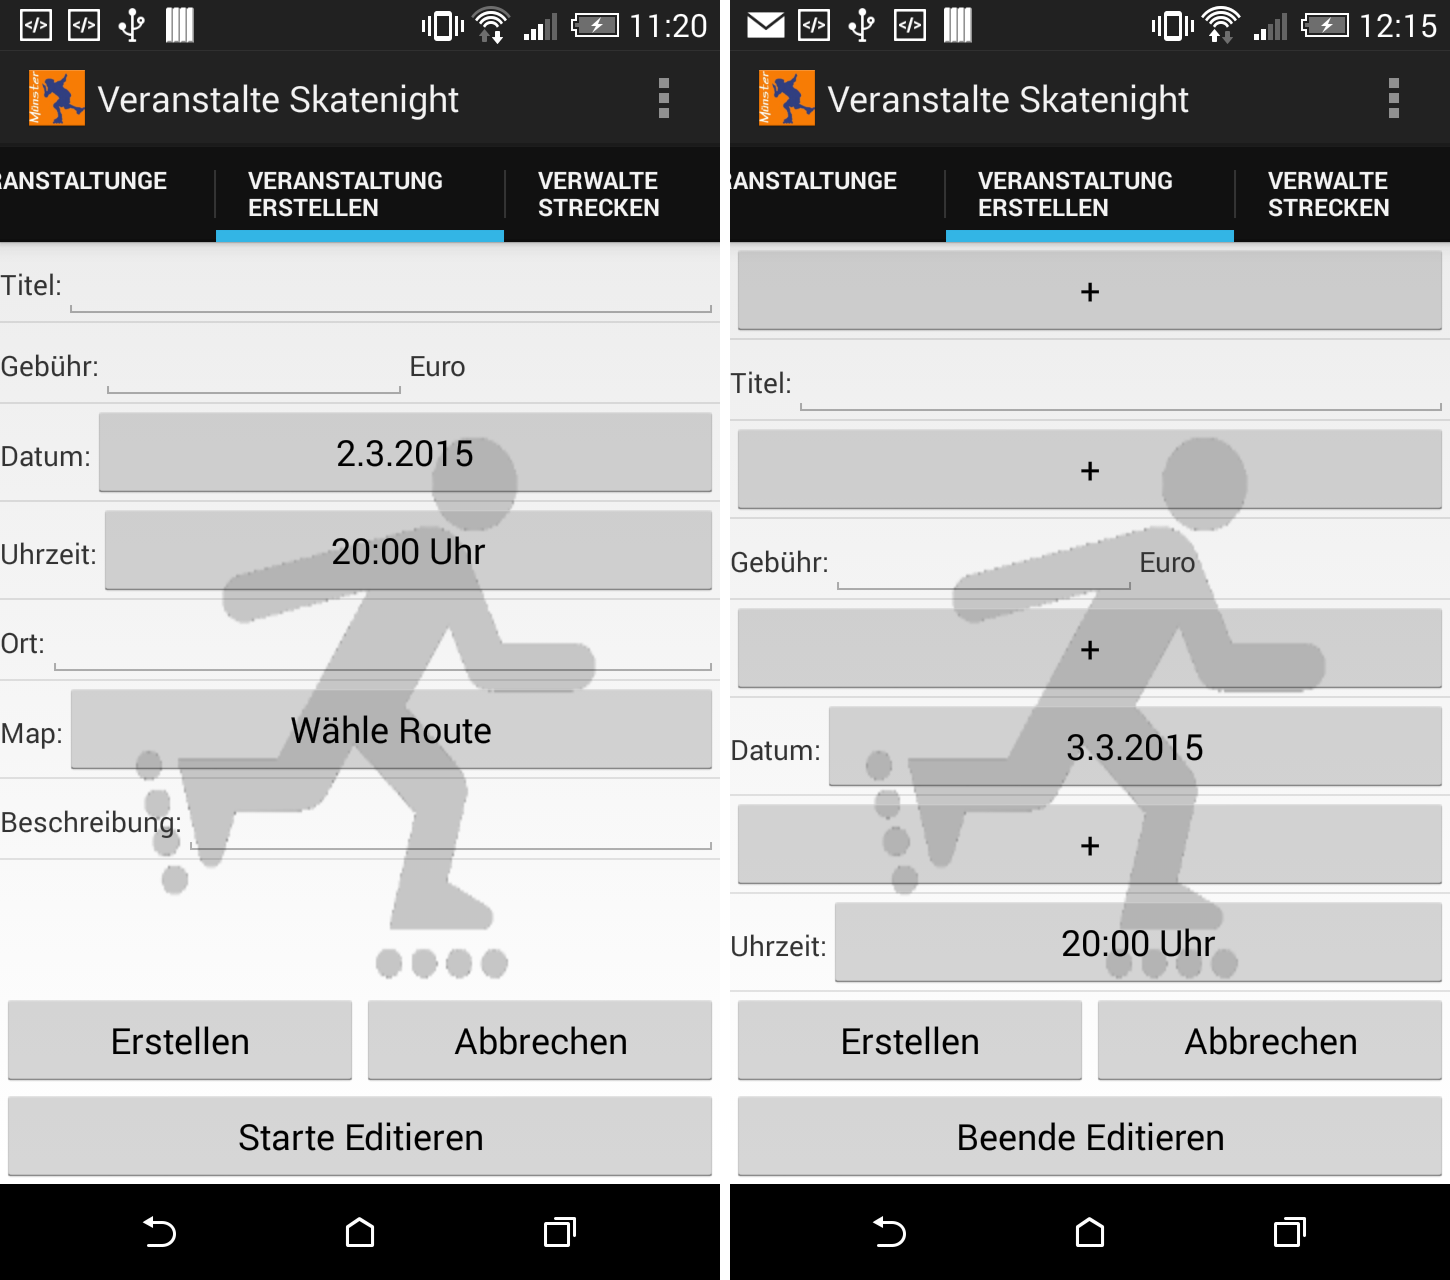
\includegraphics[width=12 cm]{graphics/Fragment_Veranstaltung_erstellen.png}
\caption{Das Fragment zur Erstellung von Veranstaltungen(links ohne, rechts mit aktiviertem Editiermodus)}
\label{fig:VeranstaltungErstellen}
\end{figure}

Vor der Einführung der 2.0 Features war die grafische Umsetzung der Erstellung einfach, da wir eine feste Anzahl von grafischen Elementen hatten, die angezeigt werden mussten um die eingegebenen Informationen vom Veranstalter zu registrieren. Nach der Einführung musste es auch möglich sein grafische Elemente zu ergänzen, da weitere Angaben, wie z.B. zusätzliche Textfelder möglich waren. Wir haben uns dazu entschieden, dies mit einer ListView und einem Adapter, dem \KLASSE{AnnounceCursorAdapter}, zu realisieren, da man einen Adapter relativ einfach um eine Datenmenge erweitern kann. Der Adapter hat als Datenmenge eine Liste von dynamischen Feldern, da diese genau eine Information zu einer Veranstaltung darstellen, und erstellt zu jedem dynamischen Feld ein grafisches View-Element und fügt es in die ListView ein. Da verschiedene Typen von dynamischen Feldern existieren, haben wir uns vor der codetechnischen Umsetzung erst verschiedene Layouts mit Hilfe von xml-Dateien erstellt, sodass der Adapter typabhängig die Layouts für die Elemente der ListView setzen kann. Damit die Felder jetzt in der ListView angezeigt werden, wird in der \METHODE{getCount}-Methode die Anzahl der angezeigten Elemente auf die Größe der Liste der dynamischen Felder gesetzt. Anschließend wird für jedes dynamische Feld die \METHODE{getView}-Methode aufgerufen, die den Typ des dynamischen Feldes an der aktuellen Position in der Liste abfragt. Wurde der richtige Typ gefunden, wird die passende Layout xml-Datei gesetzt. Die Realisierung der Erweiterung von Informationen haben wir mit einem Editiermodus gelöst. Wird der Editiermodus über den Button \glqq Starte Editieren\grqq\ gestartet erscheint über und unter jedem Element ein \glqq$+$\grqq-Button. Dazu wird in der \METHODE{getCount}-Methode im Adapter die Anzahl verdoppelt und in der \METHODE{getView}-Methode wird bei jedem zweiten Element dieser Button gezeichnet. Wird dieser gedrückt, so kann man Auswählen welches dynamische Feld an diese Stelle ergänzt werden soll. Nach der Auswahl wird die Bezeichnung des dynamischen Feldes festgelegt. Anschließend wird im Adapter die Liste mit den dynamischen Feldern um das neue Feld an der bestimmten Position ergänzt und der Adapter zeichnet die Felder neu.

Wird nun also das Fragment erstellt wird ein neues Event erstellt und die dynamischen Standard-Felder werden mit Hilfe der \KLASSE{EventUtils} in dem Event gespeichert. Dann wird der Adapter mit den dynamischen Feldern des Events initialisiert und dieser wird dann in der ListView gesetzt. Am Ende zeichnet der Adapter, wie zuvor beschrieben, die dynamischen Felder, indem er die \METHODE{getView}-Methode iteriert bis die Anzahl von der \METHODE{getCount}-Methode erreicht wird. Hat man nun alle notwendigen Informationen angegeben wird mit Hilfe der \METHODE{setEventInfo}-Methode aus den \KLASSE{EventUtils} die Informationen des Adapters an das Event übergeben. Danach wird der \KLASSE{CreateEventTask} aufgerufen, der im Hintergrund-Thread auf dem Server die neue Veranstaltung erstellt. Am Ende wird das Fragment in den Anfangszustand gesetzt und die Liste der Veranstaltungen im \KLASSE{ShowEventsFragment} wird aktualisiert.

\PARAGRAPH{Veranstaltungen editieren und löschen}
Um eine Veranstaltungen zu editieren, muss man die zu bearbeitende Veranstaltung lange berühren. Dann öffnet sich ein Menü, in dem man auswählen kann, ob man die Veranstaltung editieren oder löschen möchte. Wählt man \glqq Löschen\grqq\ so wird der \KLASSE{DeleteEventTask} aufgerufen, der die Veranstaltung im Hintergrund-Thread vom Server löscht und anschließend aus der ListView entfernt. Wählt man \glqq Editieren\grqq\ so wird ein Intent mit der \KLASSE{EditEventActivity} erstellt und dem Intent wird die ID der Veranstaltung übergeben. Anschließend wird die Activity mit dem Intent gestartet. In der Activity wird zunächst in der \METHODE{onCreate}-Methode die Veranstaltung mit der übergebenen ID vom Server  mit Hilfe der \METHODE{getEventTask} Methode abgerufen. Diese Activity sieht genau so aus wie das \KLASSE{AnnounceInformationFragment} und hat die gleiche Funktionsweise. Auch hier wird der \KLASSE{AnnounceCursorAdapter} verwendet um die Informationen der Veranstaltung anzuzeigen. Jedoch werden hier in der \KLASSE{EditEventActivity} nicht die Standard-Felder in den \KLASSE{AnnounceCursorAdapter} geladen, sondern die dynamischen Felder der abgerufenen Veranstaltung. Nun kann man wie auch schon beim Erstellen einer Veranstaltung weitere Felder über den Editiermodus ergänzen. Ist man fertig mit dem Bearbeiten der Veranstaltung und berührt den Button \glqq Speichern\grqq\ wird mit Hilfe der \KLASSE{EventUtils} die Daten der dynamischen Felder in das Event-Objekt gespeichert, das nach dem Abrufen der Veranstaltung vom Server erstellt wurde. Dann wird ein \KLASSE{EditEventTask} mit dem Event-Objekt gestartet, der die neuen Informationen der Veranstaltung im Hintergrund-Thread in das Event-Objekt auf dem Server schreibt.

\PARAGRAPH{Veranstaltungen anzeigen}
\begin{figure}[htb]
\centering
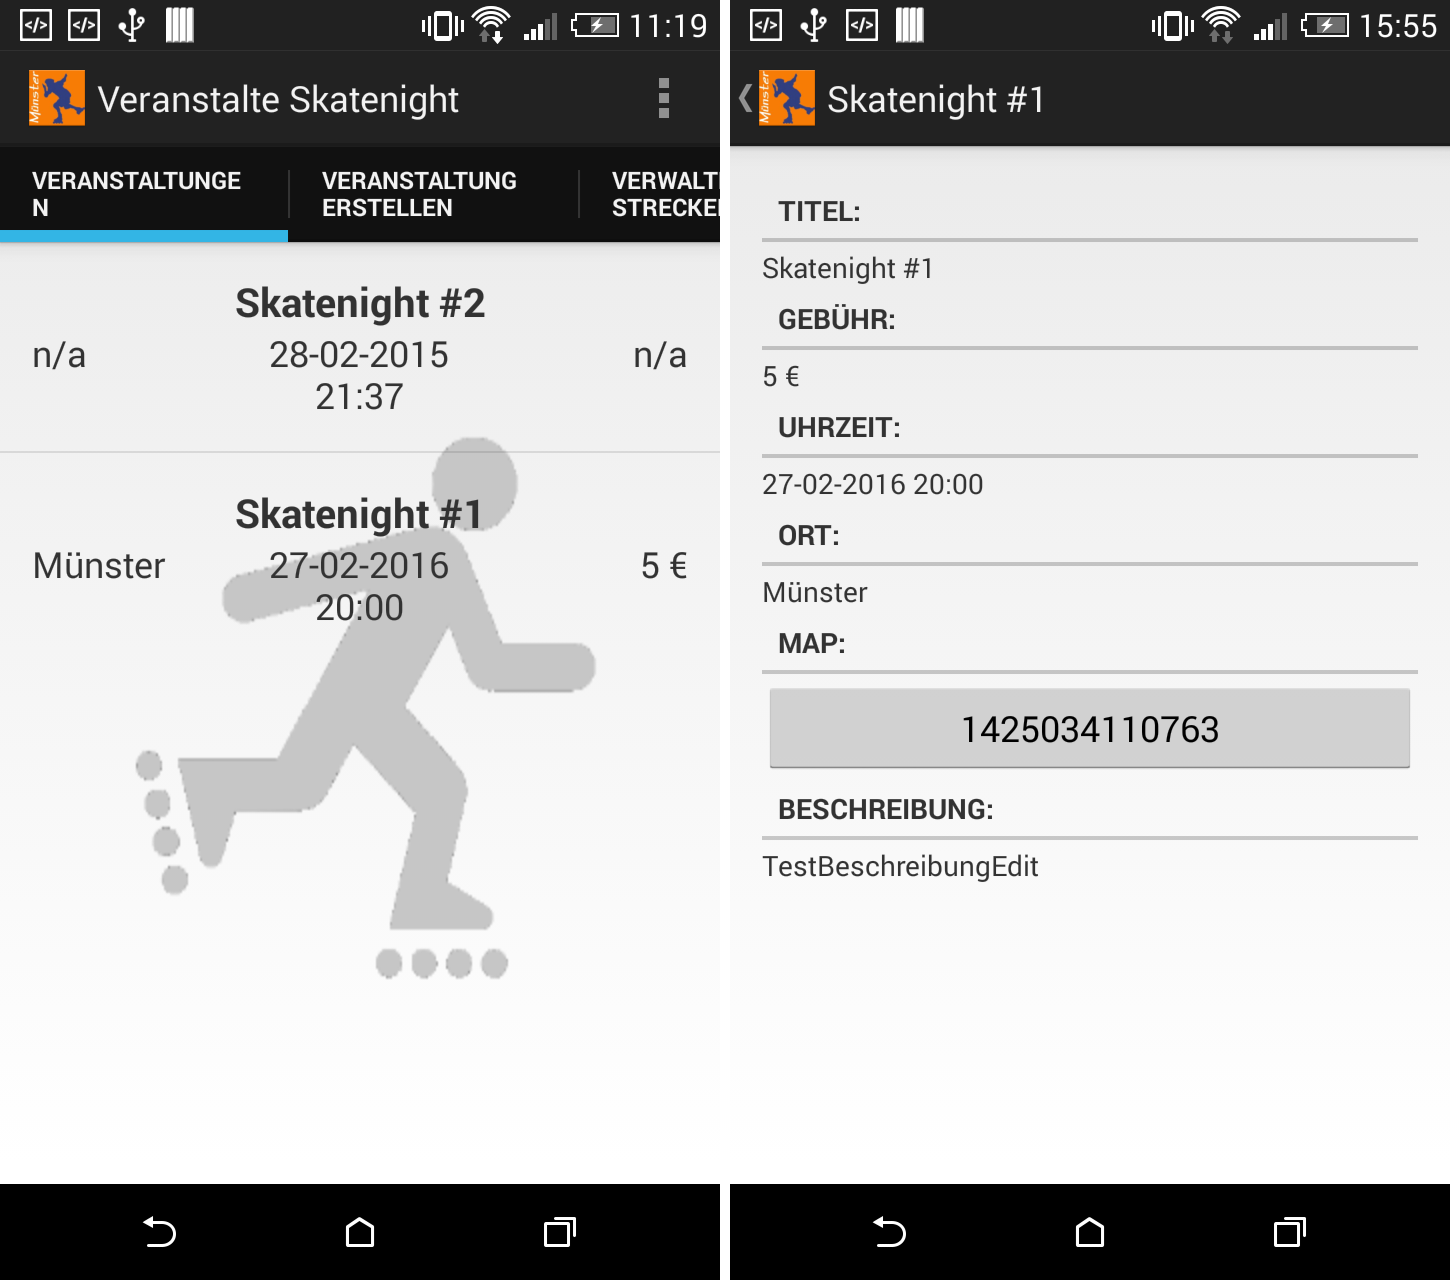
\includegraphics[width=12 cm]{graphics/show_events_veranstalter_app.png}
\caption{Anzeige von Veranstaltungen in der Veranstalter-App}
\label{fig:VeranstaltungAnzeigenVeranstalterapp}
\end{figure}

Die Veranstaltungen werden in einer ListView angezeigt, die mit einem Adapter, dem \KLASSE{EventsCursorAdapter}, mit Inhalt gefüllt wird. In der Veranstalter-App haben wir ein Fragment, das \KLASSE{ShowEventsFragment}, das die ListView anzeigt. Dieses Fragment wird geladen wenn man den ersten Tab in der Tab-Leiste auswählt und wird beim Start der App automatisch ausgewählt. Die Layout xml-Datei eines Elements der ListView enthält die wichtigsten Informationen der Veranstaltung: den Titel, der Ort, der Startzeitpunkt und die Gebühr. Wird nun das Fragment angezeigt wird der \KLASSE{QueryEventsTask} ausgeführt, der im Hintergrund-Thread die Liste der Veranstaltungen vom Server abruft. Hat der Thread seine Arbeit getan, wird ein Adapter-Objekt erstellt, die Liste der Veranstaltungen wird diesem übergeben und die ListView wird mit dem Adapter gesetzt. Anschließend wird über die \METHODE{getView}-Methode iteriert, die die passenden View-Elemente zu den Veranstaltungen erstellt und diese werden dann in der ListView angezeigt. Zusätzlich wird ein \KLASSE{OnItemClickListener} auf die ListView gesetzt, der prüft ob ein Element der ListView gedrückt wird. Wird ein Element gedrückt wird eine neue Activity, die \KLASSE{ShowInformationActivity}, gestartet. Dem Intent wird zusätzlich noch die Event-Id übergeben, da die Activity alle Informationen der Veranstaltung anzeigen soll. Da die Anzahl variabel ist, haben wir uns wieder dazu entschieden, diese Angaben in einer ListView mit einem Adapter anzuzeigen. Nach Start der Activity wird zunächst über den Intent die Event-Id ermittelt. Mit der Id wird der \KLASSE{GetEventTask} ausgeführt, der das Event-Objekt zu der Veranstaltung vom Server abruft. Abschließend wird ein \KLASSE{EventsCursorAdapter}-Objekt mit den dynamischen Feldern der Veranstaltung erstellt und diese ListView wird mit dem Adapter gesetzt. Der \KLASSE{EventsCursorAdapter} funktioniert ähnlich wie der \KLASSE{AnnounceCursorAdapter}. Wir haben wieder verschiedene Layout xml-Dateien für die verschiedenen Typen, wobei eine Layout Datei jeweils immer eine Header-TextView mit der Bezeichnung der Information hat. Dann wird in der \METHODE{getView}-Methode abgefragt um welchen Typ es sich bei dem dynamischen Feld handelt und es wird die entsprechende Layout Datei geladen und die Informationen werden gesetzt. Diese Methode wird für jedes dynamische Feld in der Liste aufgerufen. Eine spezielles dynamisches Feld ist das Feld für die Route, da in dem Fall eine Layout-Datei geladen wird, die einen Button enthält, der beim Auslösen eine neue Activity, die \KLASSE{ShowRouteActivity}, startet, die die Route der Veranstaltung anzeigt. 

\subsection{Beschreibung User-App}
\subsubsection{Gerüst}
\AUTHOR{Martin}

\begin{figure}[htb]
\centering
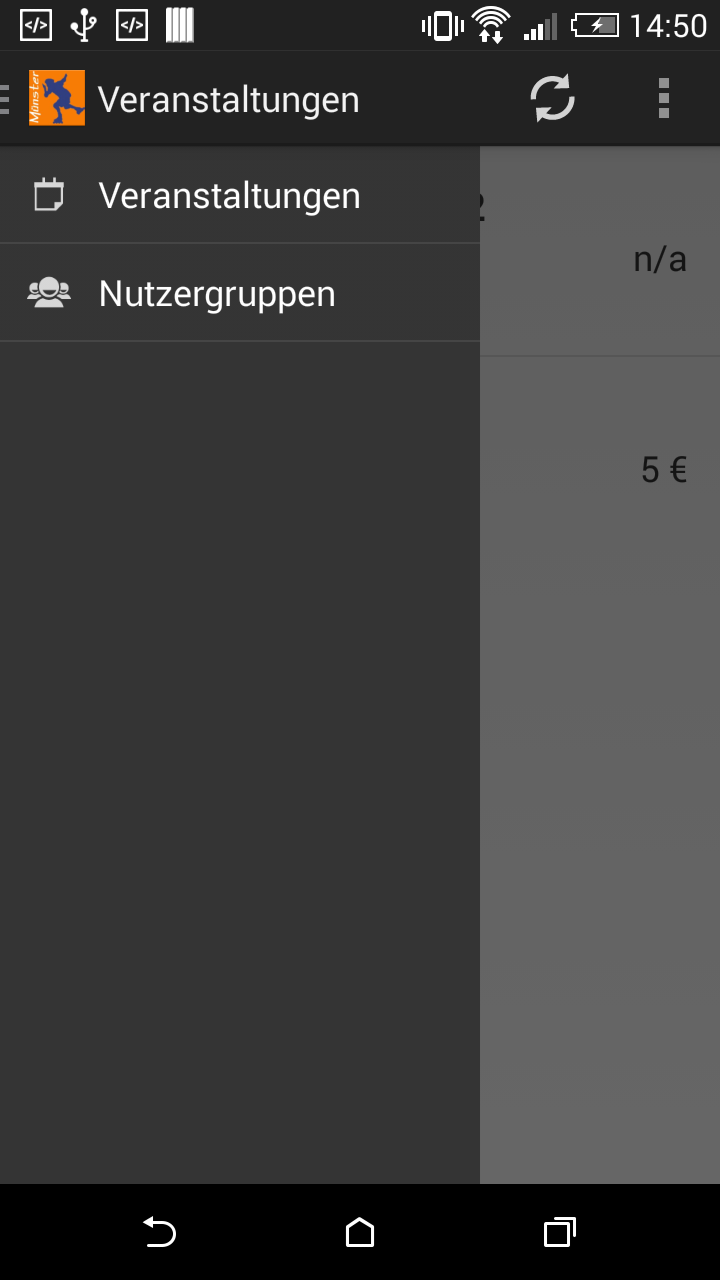
\includegraphics[width=6cm]{graphics/navigation_drawer.png}
\caption{Der ausgeklappte Navigation Drawer}
\label{fig:navigation_drawer}
\end{figure}

Die User-App besteht aus einer Activity, der \KLASSE{ShowEventsActivity}, die alle Veranstaltungen auf dem Server anzeigt und aus einer FragmentActivity, der \KLASSE{UsergroupActivitiy}, die alle Gruppen auf dem Server und alle Gruppen denen man beigetreten ist in zwei Tabs anzeigt. Um zwischen den beiden Activities zu navigieren haben wir uns entschieden einen Navigation Drawer zu verwenden. Ein Navigation Drawer ist ein Fragment, das sich von der linken Kante des Bildschirms in das Hauptfenster schiebt und die wichtigsten Navigationsmöglichkeiten der App anzeigt. Damit der Drawer angezeigt wird, muss man entweder vom linken äußersten Rand zur Mitte swipen oder das App-Icon in der ActionBar berühren. Klickt man auf eines der Felder im Navigation Drawer startet die dazugehörige Activity oder sie wird in den Vordergrund geschoben wenn bereits eine Instanz der Activity existiert. Um dies zu realisieren, haben wir eine \KLASSE{BaseActivity} und \KLASSE{BaseFragmentActivity} erstellt, die als Oberklasse jeder Activity bzw. FragmentActivity dient, die einen Navigation Drawer nutzt. In diesen Oberklassen wird die \METHODE{setContentView(int layoutResId)} Methode überschrieben. Diese Methode wird von jeder Activity in der \METHODE{onCreate}-Methode aufgerufen um das Layout zu setzen. In der überschriebenen \METHODE{setContentView}-Methode wird ein DrawerLayout geladen, in dem eine ListView existiert, die bei Start nicht sichtbar ist und außerhalb des Bildschirms liegt und ein FrameLayout, das den ganzen Platz des Bildschirms nutzt. Das Layout das von der Unterklasse mit \METHODE{setContentView} gesetzt wird, wird in dieses FrameLayout geladen sodass am Ende dann der Inhalt der Activity angezeigt wird. In der Base- bzw. BaseFragmentActivity wird in der \METHODE{setContentView}-Methode auch noch die ListView initialisiert, d.h. es werden die Menü-Titel und Menü-Icons der ListView hinzugefügt und ein ItemClickListener gesetzt, der prüft, ob ein Item berührt wurde, sodass die dazugehörige Activity geladen werden kann.
\FloatBarrier

\subsubsection{Eventanzeige}
\AUTHOR{Martin}

\begin{figure}[htb]
\centering
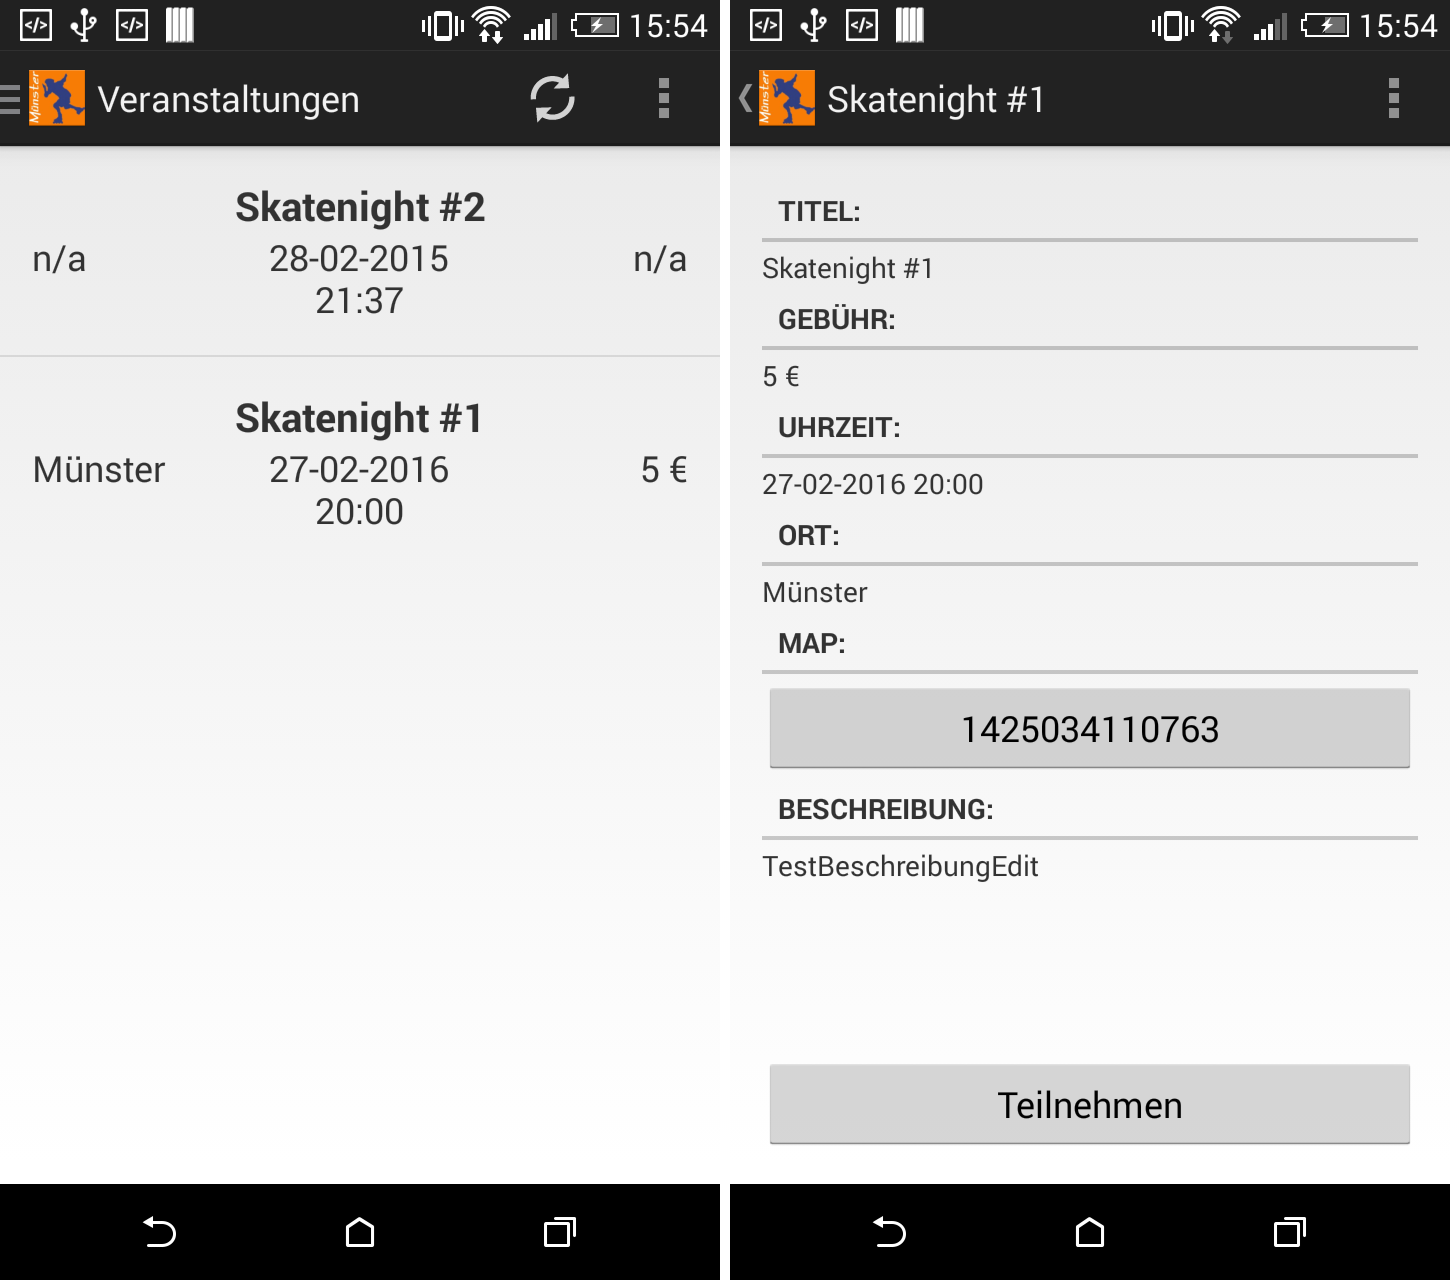
\includegraphics[width=12cm]{graphics/show_events_user_app.png}
\caption{Die Event-Anzeige der User-App}
\label{fig:show_events_user_app}
\end{figure}

Veranstaltungen werden in der User-App in der \KLASSE{ShowEventsActivity} angezeigt. Diese wird bei Start der User-App angezeigt. Zusätzlich kann man zu ihr über den Navigation Drawer navigieren. Die Anzeige der Veranstaltungen funktioniert genau so wie in der Veranstalter-App(Kapitel ...), jedoch haben wir eine Activity und kein Fragment in der die ListView angezeigt wird. Wird also die Activity gestartet, wird in der \METHODE{onCreate}-Methode die Liste der Veranstaltungen vom Server mit Hilfe des \KLASSE{QueryEventsTask} abgerufen und anschließend wird die ListView mit den Informationen gefüllt. Auch hier haben wir eine \KLASSE{ShowInformationActivity}, die gestartet wird, wenn man ein Element der ListView berührt. Die \KLASSE{ShowInformationActivity} unterscheidet sich aber in der User-App von der Veranstalter-App, da man in der User-App auch noch zusätzlich in der Activity entscheiden kann ob man an der Veranstaltung teilnehmen möchte. Dazu existiert ein Button unter der ListView, der \glqq Teilnehmen\grqq-Button, der im Fall der Teilnahme \glqq Verlassen\grqq\ heißt. Wird der \glqq Teilnehmen\grqq-Button ausgelöst, wird der Benutzer mit seiner Email-Adresse in der Veranstaltung eingetragen. Außerdem wird in dieser Activity auch die Lokale Auswertung umgesetzt. Wurde an der Veranstaltung teilgenommen und der Veranstaltungszeitpunkt wurde erreicht wird hier die lokale Auswertung geladen. Dies wird im Abschnitt der lokalen Auswertung (\ref{sec:lokaleAuswertung}) näher behandelt.
\FloatBarrier

\subsubsection{Nutzergruppen}
\AUTHOR{Bernd}

\begin{figure}[htb]
\centering
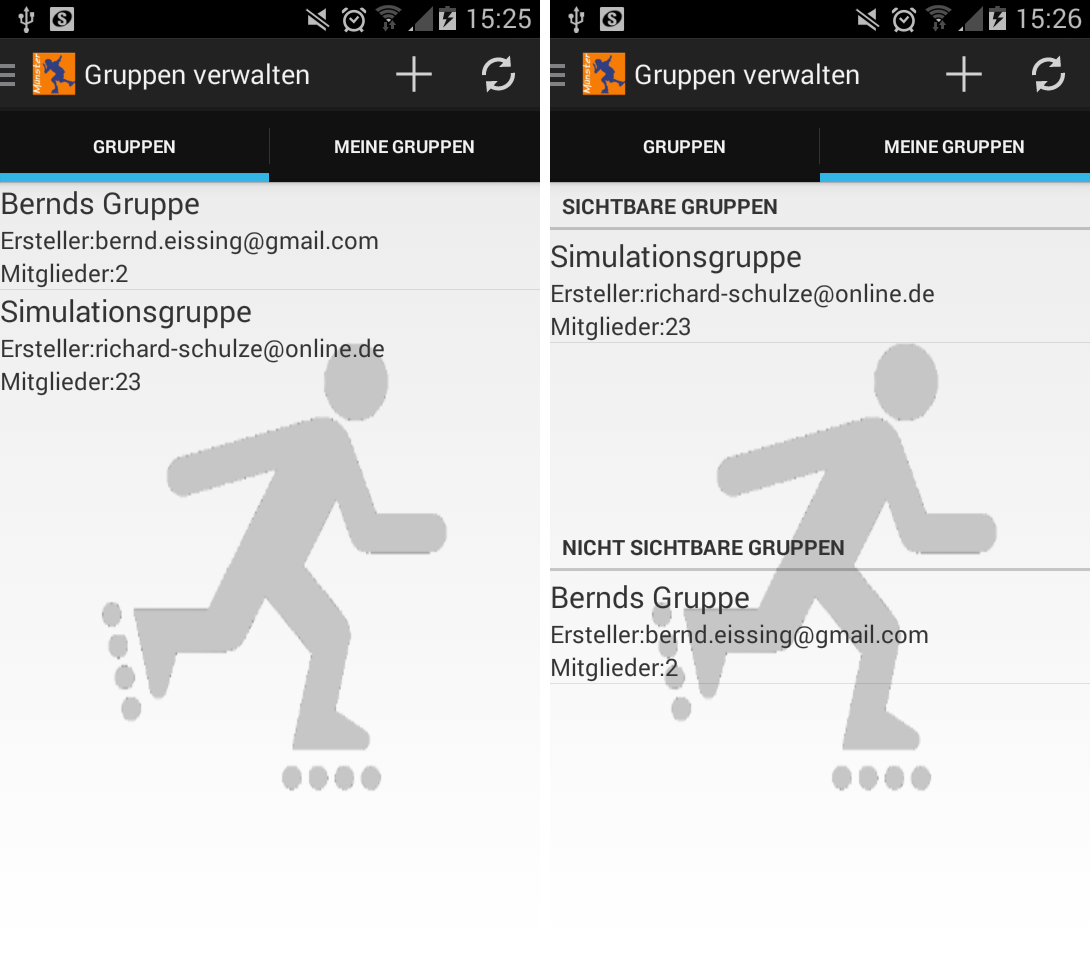
\includegraphics[width=12cm]{graphics/Usergroups_Fragments.png}
\caption{Verwaltung von Nutzergruppen}
\label{fig:usergroup_fragments}
\end{figure}

In der Userapp kann ein Benutzer eigene Nutzergruppen verwalten, anderen Nutzergruppen beitreten oder diese verlassen. Um in der Userapp zu den Nutzergruppen zu gelangen, muss der NavigationDrawer bedient werden und dort kann man dann Nutzergruppen auswählen. Die Nutzergruppen werden über eine Activity(\KLASSE{UsergroupActivity}) angezeigt, welche zwei Fragmente(das \KLASSE{AllUsergroupsFragment} und das \KLASSE{MyUsergroupsFragment}) hält. Das \KLASSE{AllUsergoupsFragment} hält eine Liste mit allen auf dem Server vorhandenen Nutzergruppen. Wenn dieses Fragment aufgerufen wird, dann wird der \KLASSE{QueryUserGroupsTask} aufgerufen, welcher in der \METHODE{doInBackground(...)} Methode alle Nutzergruppen vom Server abruft und diese dann in der \METHODE{onPostExecute(...)} Methode der ListView des Fragments hinzufügt. Der Adapter für die ListView ist der \KLASSE{UsergroupAdapter}. Dieser setzt für jede Nutzergruppe, die der ListView hinzugefügt wurden, deren Namen, Ersteller und Anzahl an Mitgliedern im Item(\DATEI{list\_view\_item\_usergroup.xml}). Der Adapter wird in der \METHODE{onResume(...)} Methode des \KLASSE{AllUsergroupsFragment} gesetzt.\\
\FloatBarrier

\PARAGRAPH{Neue Nutzergruppe erstellen}

\begin{figure}[htb]
\centering
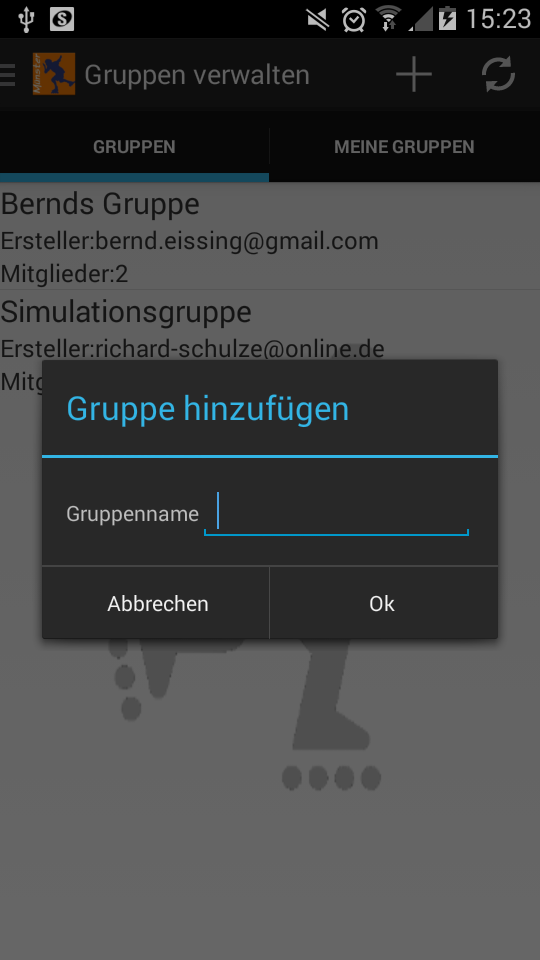
\includegraphics[width=6cm]{graphics/Nutzergruppen_neue_erstellen.png}
\caption{GUI zum Hinzufügen von Benutzergruppen}
\label{fig:usergroups_hinzufuegen}
\end{figure}

Man  hat im \KLASSE{AllUsergroupsFragment} die Möglichkeit neue Nutzergruppen zu erstellen, indem man im Optionsmenü den Plus Button betätigt. Dies führt zum Aufruf von der \METHODE{onOptionsItemSelected(...)} Methode in der  \KLASSE{UsergroupActivity}. Hier wird die \KLASSE{AddUsergroupActivity} aufgerufen, was lediglich einen Dialog darstellen soll. Die Activity hat ein Feld für den Namen der neuen Nutzergruppe, einen Button zum Abbrechen und einen Button zum Bestätigen der Aktion. Wird ein Name einer Nutzergruppe eingegeben, der nicht leer ist so wird die \METHODE{apply(...)} Methode in der \KLASSE{AddUsergroupActivity} aufgerufen. Diese Methode führt den \KLASSE{QueryUserGroupsTask} aus, welcher eine Instanz vom \KLASSE{AllUsergropusFragment} erwartet. In dem hier übergebenen Fragment wird die \METHODE{setUserGroupsToListView(...)} Methode neu definiert da diese von dem \KLASSE{QueryUserGroupsTask} in der \METHODE{onPostExecute(...)} Methode aufgerufen wird. Es werden alle Nutzergruppen nach Namen durchsucht und überprüft, ob der angegebene Name bereits vergeben ist. Ist dies nicht der Fall wird der \KLASSE{AddUserGroupTask} aufgerufen, welcher eine neue Nutzergruppe in der \METHODE{doInBackground(...)} Methode erstellt und dann die \METHODE{refresh(...)} Methode in der \KLASSE{UsergroupActivity} aufruft um die Liste mit den Nutzergruppen zu aktualisieren.
\FloatBarrier

\PARAGRAPH{Listen aktualisieren}
Die \METHODE{referesh(...)} Methode kann auch manuell aufgerufen werden, dazu muss man im Optionsmenü den Refresh Button betätigen. Die \METHODE{refresh(...)} Methode in der \KLASSE{UsergroupActivity} ruft die \METHODE{refresh(...)} Methode in dem \KLASSE{AllUsergroupsFragment} und in dem \KLASSE{MyUsergroupsFragment} auf. Dort wird der \KLASSE{QueryUserGroupsTask} im \KLASSE{AllUsergroupsFragment} und der \KLASSE{QueryMyUserGroupsTask} im \KLASSE{MyUsergroupsFragment} aufgerufen um die Liste von Nutzergruppen zu aktualisieren. 

\PARAGRAPH{Nutzergruppen beitreten und verlassen}
\label{sec:nutzergruppeBeitretenVerlassen}
Mit einem einfachen Klick auf eine Nutzergruppe in der Liste kann man dieser beitreten oder diese verlassen, solange man nicht der Ersteller ist. Beim Verlassen und beim Beitreten wird ein AlertDialog angezeigt dessen Überschrift den Namen der Gruppe darstellt zusammen mit der Frage, ob man die ausgewählte Nutzergruppe verlassen möchte und zwei Buttons zum Bestätigen und zum Abbrechen der Vorgangs. Verlässt man eine Nutzergruppe so führt dies zu zum Aufruft der \METHODE{createDialogLeave(...)} Methode in der \KLASSE{GroupUtils} Klasse. Beim Bestätigen wird der \KLASSE{LeaveUserGroupTask} mit dem Namen der ausgewählten Nutzergruppe aufgerufen. Dieser Task ruft auf dem Server die \METHODE{leaveUserGroup(...)} Methode in der \METHODE{doInBackground(...)} Methode und anschließend in der \METHODE{onPostExecute(...)} Methode die \METHODE{refresh(...)} Methode der \KLASSE{UsergroupActivity} auf, um die Änderung sichtbar zu machen. Beim Verlassen wird die \METHODE{createDialogJoin(...)} Methode in \KLASSE{GroupUtils} aufgerufen. Diese ruft bei Bestätigung den \KLASSE{JoinUserGroupTask} auf welcher die \METHODE{joinUserGroup(...)} Methode auf dem Server aufruft und abschließend die \METHODE{refresh(...)} Methode ausführt, um die Änderung sichtbar zu machen. Ist man der Ersteller der augewählten Nutzergruppe so wird die \METHODE{createDialogOwner(...)} Methode aufgerufen welche einen AlertDialog erstellt der darüber informiert, dass man der Ersteller der Nutzergruppe ist und man diese weder verlassen noch dieser beitreten kann.

\PARAGRAPH{Nutzergruppen auf der Karte sichtbar machen und löschen}

\begin{figure}[htb]
\centering
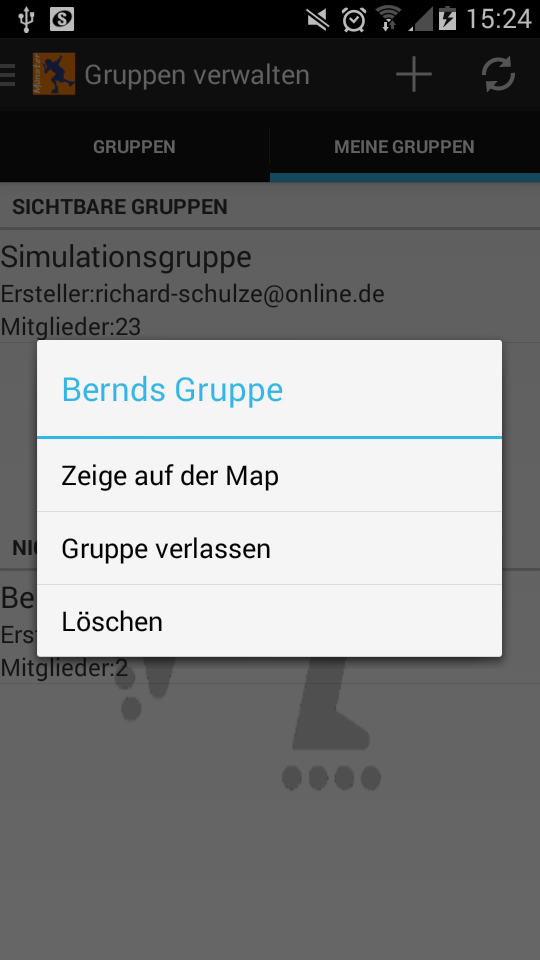
\includegraphics[width=6cm]{graphics/Nutzergruppen_selections_menu.png}
\caption{Das Auswahlmenü auf einer Gruppe}
\label{fig:usergroups_selections_menu}
\end{figure}

Das \KLASSE{MyUsergroupsFragment} enthält zwei ListViews, welche sich jeweils die Hälfte des Bildschirms teilen. Die erste ListView kann maximal fünf Nutzergruppen halten und dient dazu Nutzergruppen auf der Karte sichtbar zu machen. Die zweite ListView zeigt alle Nutergruppen an bei denen man entweder Mitglied oder Ersteller ist. Beide ListViews benutzen den \KLASSE{UsergroupAdapter} als Adapter, sie unterscheiden sich jedoch in ihren Namen. Der eine ist für die sichtbaren und der andere für die nicht sichtbaren Nutzergruppen. Mit einem Longclick auf eine Nutzergruppe in entweder der Liste der sichtbaren oder der Liste aller Nutzergruppen führt dies zu einem Aufruft der \METHODE{createSelectionsMenu(...)} Methode im \KLASSE{MyUsergroupsFragment}. Diese Methode überprüft zunächst aus welchem Adapter der Aufruft kommt und ob der Aufrufer auch gleichzeitig der Ersteller der Nutzergruppe ist. Dann wird ein AlertDialog angezeigt mit dem Namen der Nutzergruppe als Überschrift und zwei weiteren Optionen, falls man nicht der Ersteller dieser ist. Die erste Option ist es die Nutzergruppe auf der Map sichtbar oder unsichtbar zu machen. Wählt man diese Option, so wird im \KLASSE{PrefManager} die \METHODE{setGroupVisibility(...)} Methode aufgerufen, welche die Nutzergruppe sichtbar oder unsichtbar macht. Diese Methode speichert in den SharedPreferences des Smartphones die Sichtbarkeit jeder Gruppe. Die SharedPreferences sind ein lokaler Speicher der zu Key-Einträgen Werte lokal auf dem Smartphone speichert. Die zweite Option ist es die Gruppe zu verlassen; das Auswählen dieser Funktion wurde bereits in Abschnitt \ref{sec:nutzergruppeBeitretenVerlassen} erklärt. Die dritte Option ist es die Nutzergruppe zu löschen, welche nur angezeigt wird wenn man der Ersteller dieser ist. Wenn diese Option ausgewählt wird, wird die \METHODE{createDialogDelete(...)} Methode in \KLASSE{GroupUtils} aufgerufen. Hier wird ein neuer AlertDialog erstellt, dessen Überschrift der Name der Nutzergruppe ist und als Text die Frage ob man die Nutzergruppe löschen möchte zusammen mit Buttons zum Bestätigen und Abbrechen der Aktion enthält. Wird das Löschen bestätigt, so wird der \KLASSE{DeleteUserGroupTask} aufgerufen, welcher in der \METHODE{doInBackground(...)} Methode die Nutzergruppe vom Server löscht und in der \METHODE{onPostExecute(...)} Methode die Änderungen aktualisiert. 
\FloatBarrier


\subsubsection{Lokale Auswertung}
\label{sec:lokaleAuswertung}
\AUTHOR{Pascal und Daniel}

Die Lokale-Auswertung soll dem Benutzer ermöglichen statistische Daten zu erfassen, visualisieren und auszuwerten. 
Zu diesen Daten zählen: 

\begin{itemize}
	\item Der aktuelle Fortschritt auf der Strecke
	\item Die Zeit die seit dem Start des Events vergangen ist
	\item Die bereits zurück gelegte Distanz, sowie die Gesamtdistanz
	\item Die aktuelle, maximale und durchschnittliche Geschwindigkeit
	\item Die aktuelle Höhe und die zurückgelegten Höhenmeter
	\item Das Geschwindigkeitsprofil
\end{itemize}

Diese Daten sollen dem Benutzer auf intuitive Weise präsentiert werden, sodass dieser sie einfach während des Events ablesen kann. Eine besondere Herausforderung ist zu garantieren, dass die Daten unabhängig vom Status der App erfasst werden. So sollen die Daten auch aufgezeichnet werden wenn die App nicht gestartet wurde oder vorzeitig beendet wird. Des weiteren sollten sie möglichst kompakt und persistent gespeichert werden um sicherzustellen, dass die Daten auch nach Abschluss des Events analysiert werden können. Weiterhin soll die Auswertung unabhängig von der globalen Auswertung (siehe Kapitel \ref{subsec:Feldberechnung}) stattfinden, ohne die Notwendigkeit Positionsdaten an den Server zu übermitteln.

\PARAGRAPH{LocationTransmitterService}
Der \KLASSE{LocationTransmitterService} ist ein Vordergrundservice der für die Erhebung und Analyse der Positionsdaten verantwortlich ist. Dieser wird automatisch zu Beginn des Events gestartet und vom Nutzer gestoppt, sobald dieser seine Teilnahme beendet. Hier muss der Lifecycle von Services beachtet werden.  Einige unerwünschte Ereignisse könnten den Service vorzeitig beenden, was den Verlust der Daten herbeiführen würde. Um dies zu verhindern muss der \KLASSE{LocationTransmitterService} ein Vordergrundservice sein, der bei der Ressourcenfreigabe durch das System besonders berücksichtigt wird. Der Service wird um eine Notification erweitert, welche den Nutzer über seine Aktivität informiert und in Form eines \glqq Stopp\grqq\ Buttons eine Interaktion mit dem Benutzer ermöglicht (Abb. \ref{fig:LokaleAuswertungNotification}).

\begin{figure}[htb]
\centering
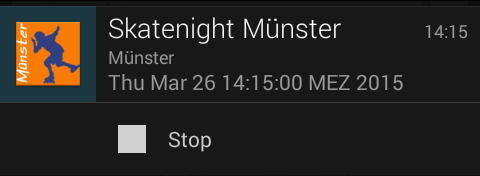
\includegraphics[width=6cm]{graphics/LokaleAuswertung_Notification.png}
\caption{Anzeige der Notification zur Kontrolle des \KLASSE{LocationTransmitterService}}
\label{fig:LokaleAuswertungNotification}
\end{figure}

Durch den Aufruf der \METHODE{startForeground(int, Notification)} Methode, mit einer einzigartigen ID und besagter Notification, wird der Service in einen Vordergrund Status versetzt. Dies geschieht nach der Initialisierung in der \METHODE{onStartCommand(Intent, int, int)} Methode des Services.

Der Service sollte ursprünglich mit Hilfe eine Push-Notification gestartet werden, dies konnte allerdings nicht verlässlich realisiert werden, da diese teilweise gar nicht oder zu häufig gesendet wurden. Um dennoch eine konsistente Datenerhebung zu gewährleisten, ohne einen Start der App vorauszusetzen, muss der Service automatisch vom System zur passenden Zeit gestartet werden. Dies ist mit Hilfe des Android AlarmManager eingeschränkt möglich. Da keine Referenzen auf registrierten Alarmzeiten gespeichert werden können, ist es nicht möglich diese nachträglich zu ändern. Da jedoch die Möglichkeit besteht, den Startzeitpunkt eines Events zu verändern, muss diese Funktionalität vorhanden sein. Gelöst haben wir dieses Problem, indem bei jeder Startzeitänderung ein neuer Alarm mit einzigartiger ID erstellt wird welche in den SharedPreferences für das Event gespeichert wird. Der ausgelöste Alarm ruft den \KLASSE{StartServiceReceiver} auf welcher zunächst überprüft ob die AlarmID mit der für das Event gespeicherten ID übereinstimmt. Ist dies nicht der Fall, so bedeutet dies eine Änderung der Alarmzeit. Es existiert also bereits ein aktuellerer Alarm. Falls der Alarm verantwortlich ist und der Service noch nicht gestartet wurde, wird dies nun erledigt.

Das betätigen des \glqq Stopp\grqq\ Buttons der Notification ruft den \KLASSE{CancelServiceReceiver} auf, welcher den Service beendet.

Der \KLASSE{LocationTransmitterService} benötigt diverse Metainformationen, wie z.B. die Routendaten und Eventinformationen, zum Ausführen der Datenanalyse. Diese werden beim Starten des Services als Extras übergeben. Zur Ermittlung der Position wird die LocationServices API der Google Play Services verwendet, bei der wir möglichst genaue Positionen im 1-Sekunden Intervall abfragen. Im Falle eines erfassten Positionswechsels ruft die LocationServices API die \METHODE{onLocationChanged(Location)} Methode des \KLASSE{LocationTransmitterService} auf.

\begin{figure}[htb]
\centering
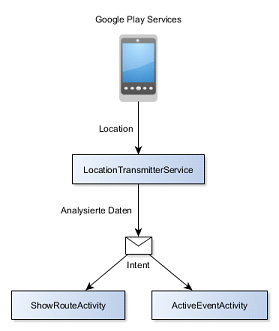
\includegraphics[width=6cm]{graphics/location_update.png}
\caption{Verarbeitung einer Positionsänderung}
\label{fig:positionsaenderung}
\end{figure}

Zunächst wird mithilfe des durch die \METHODE{calculateCurrentWaypoint(LatLng)} Methode aufgerufenen Routenpunktberechnungsalgorithmus (siehe Kapitel \ref{subsubsec:Routenpunktberechnungsalgorithmus}) der aktuelle Routenpunkt des Nutzers ermittelt und anschließend, falls sich der neu berechnete Routenpunkt vom bereits hinterlegten unterscheidet, zusammen mit der aktuellen Systemzeit, in Millisekunden seit Mitternacht des 1. Januar 1970 (UTC), abgespeichert. Nun werden die optional in der Location enthaltenen Informationen, Geschwindigkeit und Höhe, verarbeitet. Falls die Location diese Informationen enthält, wird zunächst die Geschwindigkeit von m/s auf Km/h umgerechnet und mit der bisher maximal festgestellten Geschwindigkeit verglichen. Wenn bei der Höhe eine positive Änderung erfasst wird, so wird diese Änderung zu den zurückgelegten Höhenmetern addiert. Die durchschnittliche Geschwindigkeit wird berechnet indem die bereits zurückgelegte Strecke durch die Zeit seit dem Start des Events dividiert wird. Die so ermittelten Daten werden an die registrierten BroadcastReceiver gesendet.

Beim ordentlichen Beenden des \KLASSE{LocationTransmitterService} wird dessen \METHODE{onDestroy()} Methode aufgerufen. Hier werden die erhobenen Daten in ein \KLASSE{LocalAnalysisData} Objekt überführt und anschließend mithilfe der \KLASSE{LocalStorageUtil} Klasse in den SharedPreferences persistent gespeichert. Die \KLASSE{LocalStorageUtil} verwendet hierfür die externe Bibliothek \DATEI{gson-2.2.2.jar} welche beliebige Objekte zu JSON-Strings umwandeln kann.

\PARAGRAPH{ActiveEventActivity}
Die \KLASSE{ActiveEventActivity} ist für das Anzeigen der sowohl in Echtzeit ermittelten als auch der gespeicherten Daten verantwortlich. Sie wird von der \KLASSE{ShowEventsActivity} als Alternative für die \KLASSE{ShowInformationActivity} aufgerufen, wenn das gewünschte Event bereits stattfindet und der Benutzer als Teilnehmer für dieses Event eingetragen ist. 

Da die Berechnung der Daten im  \KLASSE{LocationTransmitterService} stattfindet müssen diese lediglich in das GUI eingetragen werden. Alle Daten, bis auf die Fortschrittsanzeige, werden als einfache TextViews dargestellt, die Fortschrittsanzeige hingegen wird als Progressbar realisiert. Die beiden Buttons \glqq Geschwindigkeitsprofil\grqq\ und \glqq Karte\grqq\ rufen die \KLASSE{ShowRouteActivity} mit jeweils anderen Parametern auf.

\begin{figure}[htb]
\centering
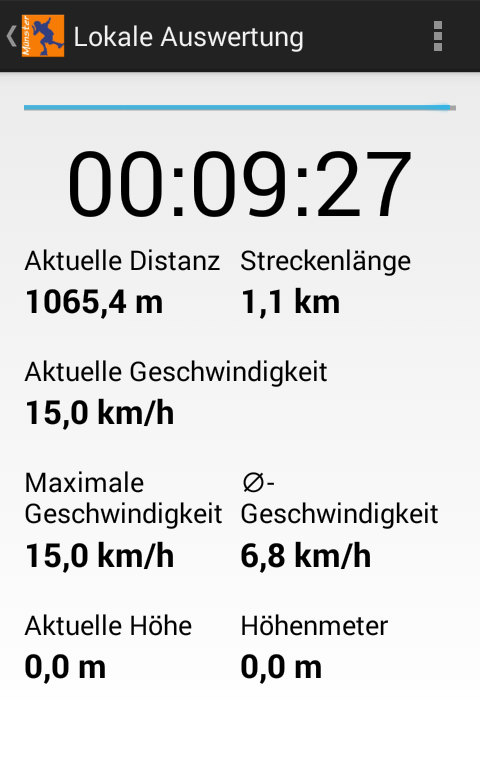
\includegraphics[width=6cm]{graphics/LokaleAuswertung.png}
\caption{Anzeige der lokalen Auswertung}
\label{fig:LokaleAuswertung}
\end{figure}

\PARAGRAPH{Geschwindigkeitsprofil}
Das Geschwindigkeitsprofil gibt sowohl Auskunft über die tatsächlich zurückgelegte Strecke, als auch über die Durchschnittsgeschwindigkeit welche der Teilnehmer zwischen den einzelnen Streckenabschnitten erreichte. Dies wird dargestellt, indem eine farbige Polyline über die besuchten Wegpunkte gelegt wird. Anhand dieser Einfärbung kann der Benutzer eine Abschätzung über sein  Geschwindigkeitsprofil treffen und zwar werden langsame Abschnitte Rot, mittelschnelle Grün und schnelle Cyan unterlegt. 

Die \KLASSE{ShowRouteActivity} welche für diese Darstellung verantwortlich ist unterscheidet zwischen einem bereits aufgezeichneten Profil und einem gerade entstehenden. Für eine bereits aufgezeichnete Strecke übergibt die \KLASSE{ActiveEventActivity} die Indizes der besuchten Routenpunkte und die dazugehörigen Zeitstempel. Diese Daten werden benötigt um das Geschwindigkeitsprofil mithilfe der \METHODE{createRouteHightlight(int[], long[])} Methode zu rekonstruieren. Wird das Profil noch aufgezeichnet, so werden stattdessen die Extras \ATTRIBUT{EventID} und \ATTRIBUT{SpeedProfile (boolean)} übergeben. In diesem Fall registriert sich die \KLASSE{ShowRouteActivity} als BroadcastReveiver für die Positionsänderungen des \KLASSE{LocationTransmitterService}. Wenn eine Positionsänderung stattfindet werden die besuchten Routenpunkte und Zeitstempel an die \KLASSE{ShowRouteActivity} weitergeleitet.

\begin{figure}[htb]
\centering
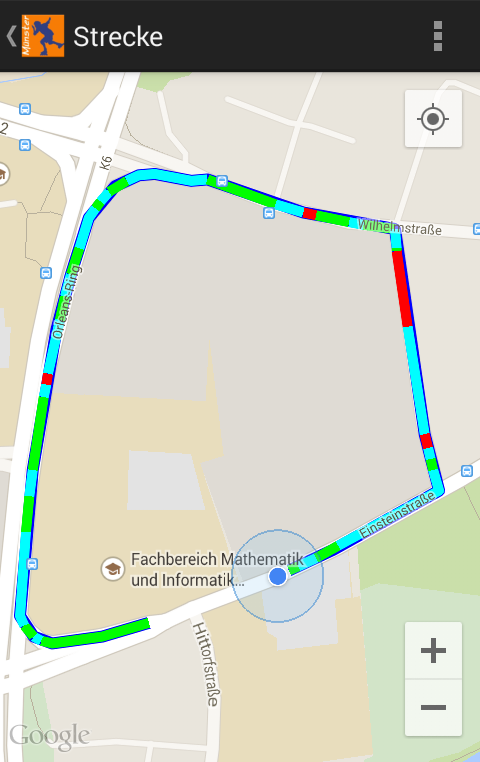
\includegraphics[width=6cm]{graphics/LokaleAuswertung_GeschwindigkeitsProfil.png}
\caption{Anzeige des Geschwindigkeitsprofils}
\label{fig:LokaleAuswertungGeschwindigkeitsprofil}
\end{figure}

Die \METHODE{createRouteHightlight(int[], long[])} Methode zeichnet den zurückgelegten Weg auf der Karte ein. Sie ermittelt mithilfe der Zeitstempel und der Distanz zwischen den Routenpunkten die Durchschnittsgeschwindigkeit des Skater. Da Polylines nur eine einzelne Farbe unterstützen, werden bei Änderung der Geschwindigkeit neue Polylines an die bereits gezeichneten angehängt. Die Methode \METHODE{colorForSpeed(float)} ermittelt die benötigte Farbe abhängig von der übergebenen Geschwindigkeit in Km/h.

\subsubsection{Einstellungen}
\AUTHOR{Tristan}
Die \KLASSE{SettingsActivity} zeigt dem Nutzer das Einstellungsmenü an. Hier kann er auswählen, ob seine Position innerhalb der App an den Server gesendet werden darf oder nicht. Zudem nutzt die \KLASSE{SettingsActivity} ein \KLASSE{PreferenceFragment}. Dies ist für Android 3.0 (API Level 11) und höher bestimmt. Für Versionen vor Android 3.0 hätte die \KLASSE{SettingsActivity} von der \KLASSE{PreferenceActivity} erben müssen, was hier jedoch nicht der Fall ist, da Fragmente eine flexiblere Architektur für die Anwendung bereitstellen im Vergleich zu der Acitivity alleine.

Das hier genutzte Fragment ist das \KLASSE{SettingsFragment}, welches das Menü über eine XML Datei \DATEI{preferences.xml} unter \DATEI{res/xml/preferences.xml} generiert.
Für die Einstellung zum Senden der eigenen Position wurde eine Checkbox verwendet, deren Standardwert auf true gesetzt ist. D.h. beim erstmaligen Starten der App ist das Senden der eigenen Position aktiviert.
Die Einstellungen werden in den \KLASSE{SharedPreferences} als boolean gespeichert unter dem Namen \glqq prefSendLocation\grqq.

\section{Testing}
\subsection{Einleitung}
\AUTHOR{Tristan}
In dem Projekt gibt es zwei Arten von Tests, die \glqq Task Tests\grqq\ und die \glqq Anwendungsfalltests\grqq\ (Use Case Tests).
Die Tasks Tests dienen hierbei zum Testen einer bestimmten Funktionalität, wie zu Beispiel dem Hinzufügen oder Löschen einer Route (\KLASSE{AddRouteTaskTest} und \KLASSE{DeleteRouteTaskTest}).
Die Anwendungsfalltests sollen im Gegensatz zu den Tasks Tests nicht nur eine Funktionalität sondern ganze Anwendungsabläufe Testen, was die UI mit einschließt.
Beide Tests, der Task Test und Anwendungsfalltest bestehen aus einem Konstruktor zum Initialisieren oder Aufsetzen der Testdaten, welcher einmalig im Test aufgerufen wird und einer \METHODE{setUp}-Methode, die vor jedem einzelnen Test aufgerufen wird. Sie dient dazu Variablen zu initialisieren und Daten von vorherigen Tests \glqq aufzuräumen\grqq. Weiterhin gibt es  bei dem Task Test eine einzige Methode, die ausschließlich die Funktion testet, für die der Test bestimmt ist (\METHODE{testTask()}-Methode).

\subsection{Funktionsweise der Anwendungsfalltests}
\AUTHOR{Tristan}
Da die TaskTests an anderer Stelle genauer beschrieben werden und nicht die Komplexität der Anwendungsfalltests aufweisen, wird hier der allgemeine Ablaufe sowie die Funktionsweise dieser Tests genauer beschrieben.

Einfachheitshalber werden die Anwendungsfalltests ab jetzt nur noch als Tests bezeichnet und beziehen sich nur auf diesen Abschnitt. Die Testklassen verwenden als \glqq Base Test Case Class\grqq\ die \KLASSE{ActivityInstrumentationTestCase2} Klasse, welche Methoden zur Interaktion mit der UI unter Testbedingungen zur Verfügung stellt und in dem Paket \glqq android.test\grqq\ enthalten ist.
Der Test erbt also von dieser Klasse. Zusätzlich wird hierbei die Activity angegeben, in der der Test starten soll. Zum Beispiel startet der Test bei \KLASSE{ActivityInstrumentationTestCase2<HoldTabsActivity>} in der \KLASSE{HoldTabsActivity}. Zudem ist die Reihenfolge, in der die Tests ausgeführt werden nicht vorgegeben und kann variieren.

\subsubsection*{Konstruktor}
Weiterhin wird im Konstruktor lediglich der superclass Konstruktor auf gerufen und die Klasse der Start Activity übergeben (HoldtabsActivity.class).

\subsubsection*{setUp Methode}
Die \METHODE{setUp}-Methode wird vor jedem Test aufgerufen und dient wie bereits erwähnt der Initialisierung und dem Löschen der Testdaten vorheriger Tests, da ein Anwendungsfall mehrere Test Methoden enthalten kann. Zuerst wird die superclass-Methode aufgerufen (super.setUp) und anschließen folgt der Initialisierungscode. Um die UI ohne Fehler von außen Testen zu können wird der Touch Mode mit \METHODE{setActivityInitialTouchMode(false)} ausgeschaltet. In der Regel wird hier auch die Activity gestartet, falls dies noch nicht der Fall sein sollte (\METHODE{getActivity()}) und einem Klassenattribut \ATTRIBUT{mActivity} zugewiesen.

\subsubsection*{testPreConditions Test}
Stellt sicher, dass die Vorbedingungen für die Anwendung fehlerfrei initialisiert wurden. Dazu gehören unter anderem die UI Elemente und das Starten der Activity.

\subsubsection*{testUseCase Test}
Alle Tests, die auch die UI Testen, laufen auf einem extra dafür vorgesehen Thread, dem UiThread. Auf diesem werden alle Interaktionen wie Buttonklicks oder Swipen simuliert. In den meisten Fällen werden Key Events simuliert mit \METHODE{sendKeys} in dem UIThread und anschließen folgt die Überprüfung mit Hilfe von \glqq Asserts\grqq\ wie in Junit. Diese prüfen, ob die Werte zum Beispiel die über den UI Thread eingegebenen Daten in Editfelder mit den erwarteten Werten übereinstimmen. Ist dies der Fall fährt der Test fort und endet, wenn alle Asserts fehlerfrei waren. Sollte jedoch ein Assert fehlschlagen, wird die Methode \METHODE{testUseCase} abgebrochen und gilt somit als nicht bestanden. Außerdem können innerhalb des Tests auch andere Activities gestartet werden. Diese laufen dann über einen \KLASSE{Instrumentation.ActivityMonitor} über den die gestartete Activity überwacht wird, anschließen wird der Test Code ausgeführt und die Activity wieder geschlossen mit dem Befehl \METHODE{finish()}. Sollte diese Activiy an dieser Stelle nicht über \METHODE{finish()} beendet werden und der \METHODE{testUseCase()} erfolgreich abgeschlossen worden sein, läuft diese Activity im Hintergrund über den Monitor weiter und kann zu fehlerhaften Ergebnissen in anderen Tests führen.

\subsubsection*{State Management Tests}
Diese Art von Tests verifizieren die Activity in den Status \glqq Pausieren\grqq\ oder \glqq Beendet\grqq. Folglich das Verhalten der Activity nach dem Fortsetzen oder Neustarten. Diese Art von Tests sind nicht in allen Anwendungsfalltests enthalten.
Der Test \METHODE{testStateDestroy} verwendet die von der Klasse \KLASSE{InstrumentationTestCase2} bereit gestellte Methode \METHODE{finish()} (\METHODE{mActivity.finish()}) zum Beenden der Activity und der Test \METHODE{testStatePause} die Methoden \METHODE{callActivityOnPause} und \METHODE{callActivityOnResume}. Diese halten die App an, was beispielsweise ein Klick des Nutzers auf den \glqq Home Screen Button\grqq\ sein könnte.

Innerhalb des Tests wurde häufiger der Befehl \METHODE{Thead.sleep(Zeitangabe)} verwendet, was den Hintergrund hat bei zeitkritischen Abschnitten eine bestimmte Zeit lang zu warten, damit zum Beispiel Daten vom Server über Netzwerkverbindungen, UI Elemente rechtzeitig initialisiert werden (die Zeit kann Testgeräte abhängig sein) oder die GPS Position ermittelt werden kann.

Auch kommen in den Testklassen die Begriffe \glqq Small\grqq, \glqq Medium\grqq\ und \glqq Large\grqq\ – Test vor. Deren Zweck ist es über den \glqq Scope\grqq, Abhängigkeiten und Performance Faktoren der Tests zu informieren, die Code-Qualität sowie System Instandhaltung zu verbessern.

\textbf{Small (Unit):} Verifiziert kleine \glqq low-level\grqq\ Logik meist im Bereich einer Methode oder Klasse und bezieht sich auf keine externen Ressourcen. Die Ausführungszeit sollte im Sekunden (besser Millisekunden) Bereich liegen.

\textbf{Medium (Integration):} Kann mehrere Interaktionen zwischen Komponenten enthalten und auch auf externe Datei Systeme zugreifen oder mehrere Prozesse laufen lassen. Die Ausführungszeit kann Minuten betragen (vorzugsweise Sekunden).

\textbf{Large (System):} Hier kann es sein das der Test auch auf externe Ressourcen, wie Server über das Internet zu greifen muss. Die Ausführungszeit kann hier also etwas länger betragen, von Sekunden, Minuten oder Stunden.

\subsection{Simulator}
\AUTHOR{Richard}
Zu besseren Testbarkeit der App ist während der Entwicklung auch ein Simulator für eine Skatenight entstanden. Der Simulator ist in JavaScript geschrieben und benutzt JQuery, sowie die Google Maps API v3 als Bibliotheken.

Im Quelltext des Simulators kann in Zeile 50 die Adresse des Backends eingegeben werden, dass zur Simulation genutzt werden soll. So hat man die Möglichkeit, nicht nur auf dem Debug-Server sondern auch auf dem Jenkins- und Release-Server Felder zu simulieren. Nach dem Starten des Simulators werden dann die Events des entsprechenden Servers automatisch heruntergeladen und in dem Dropdown-Menü angezeigt. Wenn ein Event ausgewählt wird, wird die Strecke des Events als roter Polygonenzug auf der Karte dargestellt. Es kann unterhalb der Dropdownliste angegeben werden, wieviele Skater simuliert werden sollen, wie schnell sie fahren, wie groß das Feld ist, also auf welcher Fläche sie sich verteilen sollen, und in welchen Abständen die Position der Skater auf den Server übertragen werden soll. Mit den Schaltfläche \glqq Start\grqq, \glqq Pause\grqq\ und \glqq Stop\grqq\ kann die Simulation gesteuert werden.

Zur Simulation der Skater wird auf dem Server die Methode \METHODE{simulateMemberLocations} aufgerufen. Diese nimmt die Positionen für viele Skater gleichzeitig entgegen und ruft anschließend jeweils die eigentliche Methode zur Aktualisierung der Position \METHODE{updateMemberLocation} auf. Wir haben uns für diese Lösung entschieden, da Probleme auftraten, wenn der Simulator direkt die \METHODE{updateMemberLocation}-Methode nutzte. Die zu große Anzahl Anfragen hat den kostenlosen Rahmen der Google App Engine innerhalb einer sehr kurzen Zeit aufgebraucht. Über die Methode zur Simulation der Positionen wird unabhängig von der Anzahl der Skater immer nur eine Anfrage gestellt.

\subsection{Task-Tests}
\AUTHOR{Bernd}
Fast alle TaskTests befinden sich in der Veranstalterapp angefangen mit dem \KLASSE{AddRouteTaskTest}. Dieser Test erstellt eine neue Route und löscht als Vorbereitung alle Routen und Veranstaltungen vom Server. Im eigentlichen Test wird dann die erstellte Route mit dem \KLASSE{AddRouteTask} dem Server hinzugefügt und es wird geprüft, ob diese dann auf dem Server gespeichert ist, indem die \METHODE{getRoutes(...)} Methode auf dem Server aufgerufen wird.

Der \KLASSE{CreateEventTaskTest} ist ähnlich wie der AddRouteTaskTest. Er erstellt eine Route, eine Veranstaltung und fügt der Veranstaltung die Route hinzu, da Veranstaltungen nicht ohne Routen gespeichert werden können. Als Vorbereitung werden auch hier alle Routen und Veranstaltungen gelöscht und es wird auf dem Server die \METHODE{addRoute(...)}  Methode und die \METHODE{createEvent(...)} Methode aufgerufen. Im eigentlichen Test wird dann auf dem Server der \KLASSE{QueryEventTask} aufgerufen, um die erstellte Veranstaltung zu überprüfen. 

Der \KLASSE{DeleteEventTaskTest} erstellt eine Route und zwei Veranstaltungen. Als Vorbereitung werden wieder alle Veranstaltungen und Routen vom Server gelöscht und dann die beiden Veranstaltungen mit der Route auf dem Server gespeichert. Im eigentlichen Test wird dann eine Veranstaltung vom Server durch Aufrufen des \KLASSE{DeleteEventsTasks} gelöscht und es wird überprüft, ob die übrig gebliebene Veranstaltung die richtige ist.

Der \KLASSE{DeleteRouteTaskTest} erstellt drei Routen und als Vorbereitung werden alle Routen und Veranstaltungen vom Server gelöscht und die drei Routen dem Server hinzugefügt. Im eigentlichen Test wird dann eine Route vom Server durch Aufrufen des \KLASSE{DeleteRouteTasks} gelöscht und es wird geprüft, ob die gelöschte Route noch auf dem Server vorhanden ist. Dies geschieht, indem auf dem Server die \METHODE{getRoutes(...)} Methode aufgerufen wird und die erhaltene Liste von Routen auf die gelöschte Route untersucht wird.

Der \KLASSE{EditEventTaskTest} erstellt eine Veranstaltung und zwei Routen. Als Vorbereitung werden alle Veranstaltungen vom Server gelöscht und die neue Veranstaltung dem Server hinzugefügt. Im eigentlichen Test werden die Daten der angelegten Veranstaltung geändert und es wird der \KLASSE{EditEventTask} aufgerufen. Abschließend werden die veränderten Daten der Veranstaltung überprüft. 

Der \KLASSE{GetEventTaskTest} erstellt eine Veranstaltung und eine Route. Als Vorbereitung werden alle Veranstaltungen vom Server gelöscht und die neue Veranstaltung dem Server hinzugefügt. Im eigentlichen Test wird dann die \METHODE{getEvent(...)} Methode auf dem Server aufgerufen und die Daten der erhaltenen Verantstaltung mit der erstellten verglichen. Abschließend werden alle Routen und Veranstaltungen vom Server gelöscht.

Der \KLASSE{QueryEventTaskTest} erstellt zwei Veranstaltungen und zwei Routen. Als Vorbereitung werden alle Veranstaltungen und Routen vom Server gelöscht und die beiden Veranstaltungen mit den beiden Routen auf dem Server gespeichert. Im eigentlichen Test werden dann alle Veranstaltungen vom Server mit dem \KLASSE{QueryEventTask} abgefragt und es wird überprüft, ob die erhaltene Liste von Veranstaltungen die beiden erstellten Veranstaltungen beinhaltet. Abschließend werden alle Veranstaltungen und Routen vom Server gelöscht. 

Der \KLASSE{QueryRouteTaskTest} erstellt drei Routen. Als Vorbereitung werden alle Routen und Veranstaltungen vom Server gelöscht und die drei erstellten Routen dem Server hinzugefügt. Im eigentlichen Test werden die Routen vom Server abgefragt indem der \KLASSE{QueryRouteTask} aufgerufen wird und die erhaltene Liste von Routen auf die drei erstellten Routen untersucht wird. Abschließend werden alle Routen vom Server gelöscht.

\subsection{Use-Case-Tests: Veranstalter-App}
\subsubsection{AddAndDeleteHostTest}
\AUTHOR{Bernd}

\subsubsection{AuthenticationOrganizerTest}
\AUTHOR{Bernd}

\subsubsection{CreateAndDeleteRouteTest}
\AUTHOR{Richard}
Der \KLASSE{CreateAndDeleteRouteTest} legt, wie der Name schon sagt, eine Route an und löscht sie anschließend wieder. Da es sich um einen Use-Case-Tests handelt, werden die Abläufe vollständig über die GUI gesteuert. Lediglich beim Löschen der Route wird nicht über die GUI-Elemente das Löschen angestoßen, sondern direkt die entsprechende Methode auf dem Fragment zur Verwaltung der Routen aufgerufen. Dies ist notwendig, da wir in den Tests das Auswählen von Optionen in einem Kontextmenü nicht an allen Stellen simulieren konnten. Der weitere Ablauf des Löschens wird aber exakt wie in der Veranstalter-App abgearbeitet.

Im Test wird nach einer kurzen Wartezeit in der initialisierten View auf den Plus-Button im \KLASSE{ManageRoutesFragment} gedrückt. Es öffnet sich dadurch der Dialog, der den Namen der neuen Route entgegennimmt. Nach Eintragen eines Teststrings, wird mit der OK-Taste bestätigt und es öffnet sich der Routeneditor. Nach einer erneuten Wartezeit ist die Route vollständig geladen und es werden zwei Wegpunkte über den Plus-Button in der ActionBar erstellt. Nach Erstellung des ersten Wegpunktes wird die Karte ein Stück verschoben, damit sich der zweite Wegpunkt an einer anderen Position befindet. Durch die Simulation eines Zurück-Tastenklicks wird der Sicherungsdialog angezeigt, der bestätigt und damit geschlossen wird. Der Test wartet dann, bis die neue Route angelegt wurde und löscht diese über den bereits erwähnten Aufruf beim \KLASSE{ManageRoutesFragment}.

\subsubsection{PublishNewInformationTest}
\AUTHORNOSPACE{Tristan}
\paragraph{Anwendungsfallbeschreibung:} Veröffentlichen neuer Informationen 2.0

\textbf{Beteiligte Akteure:}
	Veranstalter
	
\textbf{Anfangsbedingungen:}
	Der Veranstalter hat die Veranstalter-App geöffnet, ist bereits eingeloggt und befindet sich in der \KLASSE{HoldTabsActivity} auf dem Veranstaltungen Tab.
	
\textbf{Ereignisfluss:}
	\begin{enumerate}
		\item Es wird  auf das Tab zum Event erstellen geswipet.
		\item Es werden alle Felder für das Event ausgefüllt bzw. neue Eigenschaften hinzugefügt.
		\item Über \glqq Erstellen\grqq\ wird das Event erstellt.
		\item Die Erstellung wird über einen Dialog nochmal bestätigt.
		\item Ab dem ersten Schritt wiederholen, um mehrere Events anzulegen.
		\item Es wird zu dem Veranstaltungen Tab geswipet.
		\item Von den angezeigten Events wird eines ausgewählt.
		\item Es wird ein Menü zur Bearbeitung des ausgewählten Events angezeigt.
		\item Bereits existierende Informationen können bearbeitet oder über den Button \glqq Editiere Event Eigenschaften\grqq\ neue Eigenschaften hinzugefügt werden.
		\item Das Event wird über den Speichern Button editiert.
	\end{enumerate}
	
\textbf{Abschlussbedingungen:}
	Neue Veranstaltung anlegen und diese anschließend editieren.
	
\textbf{Ausnahmen:}
	Keine
	
\textbf{Spezielle Anforderungen:}
	Internetverbindung

\paragraph{Testablauf:}
Vorbedingung für den Test ist eine bestehende Internetverbindung, damit das anzulegende Event auf dem Server gespeichert werden kann.
Die Test Daten für die Klasse sind als private, statische sowie konstante Member der Klasse definiert (\ATTRIBUT{TEST\_TITLE} etc.). Dabei sind die Daten mit dem Präfix \glqq TEST\_\grqq\ für den normalen useCase Test und \KLASSE{StatePauseResume} Test vorgesehen und die mit dem Präfix \glqq TEST\_STATE\_DESTROY\grqq\ für den StateDestroy Test. Zudem sind die UI Elemente als private Member deklariert.
Der Test läuft über die \KLASSE{HoldTabsActivity} der \glqq VeranstalterApp\grqq. Das hier angelegte Test Event wird an anderer Stelle in einem Test der User-App \KLASSE{ShowServeralEventsTest}  verifiziert und wird somit nach Beendigung des Tests nicht gelöscht.

\textbf{setUp():} Hier wird für den Nutzer das Google Konto ausgewählt zu Authentifizierung, zum \glqq Veranstaltungen Erstellen\grqq\ Tab geswipt sowie die App gestartet.

\textbf{Swipe(Direction):} Da die InstrumentationTestCase2 Klasse keine Methoden zum swipen für das wechseln der Tabs bereitstellt, wird diese Funktionalität hier definiert. Es kann entweder right oder left (privates enum) der Klasse übergeben werden und führt dann die entsprechende Tätigkeit aus.

\textbf{testViews():} Activity, Testet, ob alle UI Elemente, Edits, Buttons, TimePicker etc. initialisiert wurden in der setUp Methode mit Hilfe von assertNotNull(UIElement).

\textbf{testViewsVisible():} Verifiziert lediglich ob die Elemente auch auf dem Smartphone Screen sichtbar sind (assertOnScreen bereitgestellte Methode der InstrumentationTestCase2).

\textbf{testPreConditions():} Prüft, ob alle Tabs in der ActionBar (mActionBar) enthalten sind.

\textbf{testUseCase():} Kann eine Exception werfen auf Grund des UI Threads. Hier wird der Anwendungsfall verifiziert. Hierzu wird auf das Tab zum erstellen geswipt, die Test Daten eingegeben und abgebrochen um auch diese Funktionalität zu testen. Danach werden die Test Daten erneut eingegeben und auf den \glqq Erstellen\grqq\ Button gedrückt und mit einem auftauchenden Dialog nochmal bestätigt wird. Es wird geprüft, ob das Event auf dem Server gespeichert wurde. Danach wird zu den Veranstaltungen Tab geswipt und das eben angelegt Event mit einem Long Touch zum Editieren ausgewählt. Die Testen zum Editieren werden eingegeben und wie vorhin wird Bestätigt und zu dem Veranstaltung Tab geswipt sowie geprüft, ob das editierte Event auch auf dem Server gespeichert wurde.

\textbf{State Tests:} Hier wird getestet, ob die Daten beim Beenden der App aus den Eingabefelder gelöscht werden, falls welche beim Erstellen schon eingegeben worden sind oder bestehen bleiben, beim Pausieren der App.

\textbf{Anmerkung:} Die weiteren Tests \KLASSE{SendCurrentPositionTest}, \KLASSE{SendPositionSettingsTest} und \KLASSE{ShowSeveralEventsTest} werden nicht so genau geschrieben, sondern auf JavaDoc und Inline Kommentare verwiesen.


\subsection{Use-Case-Tests: User-App}
\subsubsection{CreateJoinLeaveDeleteUserGroupTest}
\AUTHOR{Bernd}
Dieser Test ist ein Use-Case in dem eine Nutzergruppe erstellt wird, einer anderen Nutzergruppe, bei der man noch nicht Mitglied ist, beigetreten wird, diese dann wieder verlässt und die erstellte Nutzergruppe zum Schluss wieder gelöscht wird. Damit dieser Test funktioniert muss vor Ausführung schon eine Nutzergruppe existieren, bei der der auf dem Testhandy angemeldete Benutzer nicht schon ein Mitglied ist. Des weiteren darf noch keine Nutzergruppe mit dem Namen \glqq TestGroup\grqq\ auf dem Server existieren.

Zu Beginn des Tests wird der Benutzer mit dem Server verbunden, das heißt es wird seine E-Mail an den Server gesendet und es wird die \KLASSE{UsergroupActivity} gestartet. Im ersten Teil des Tests werden die Views getestet, das heißt es wird geprüft, ob sowohl die ActionBar als auch der sich darauf befindende Plus Button richtig referenziert wurden. Im zweiten Teil beginnt der Use-Case, in dem als erstes ein Klick auf den Plus Button simuliert wird. Es wird dann so lange gewartet, bis sich die \KLASSE{AddUserGroupActivity} gestartet hat und dort wird dann in das Feld für die Nutzergruppe der Name \glqq TestGroup\grqq\ eingetragen und es wird ein Klick auf den \glqq Ok\grqq-Button simuliert. Es wird dann wieder auf die \KLASSE{AddUserGroupActivity} gewartet und in der ListView vom \KLASSE{AllUsergroupsFragment} nach der Nutzergruppe mit dem Namen \glqq TestGroup\grqq\ gesucht. Ist die Suche erfolglos so schlägt der Test fehl, bei erfolgreichem Suchen läuft der Test weiter. Als nächstes wird die ListView nach einer Nutzergruppe durchsucht, bei der der Benutzer noch nicht als Mitglied eingetragen ist. Ist keine vorhanden, so schlägt der Test mit einer Fehlermeldung fehl. Ist eine Nutzergruppe vorhanden, bei der der Benutzer noch kein Mitglied ist so wird ein Klick auf die Stelle in der ListView simuliert, bei der die Nutzergruppe gefunden wurde. Dies startet dann einen AlertDialog zum beitreten einer Nutzergruppe. Es wird so lange gewartet, bist der Dialog angezeigt wird. Es wird ein Klick auf den Ja Button simuliert um der Nutzergruppe beizutreten. Darauf hin wird überprüft, ob der Bediener nun in der Liste von Mitgliedern der soeben beigetretenen Nutzergruppe enthalten ist. Ist dies nicht der Fall, so schlägt der Test fehl ansonsten läuft der Test weiter. Nun wird ein Klick auf die Stelle in der ListView simuliert, bei der sich die Nutzergruppe befindet der man soeben beigetreten ist. Auch hier wird ein AlertDialog zum Verlassen der Nutzergruppe angezeigt. Es wird wieder so lange gewartet, bis der AlertDialog erscheint. Hier wird wieder ein Klick auf den Ja Button simuliert um die Nutzergruppe zu verlassen. Nun wird überprüft, ob der Benutzer in der Liste von Mitgliedern der Nutzergruppe enthalten ist. Ist dies der Fall so schlägt der Test fehl ansonsten läuft der Test weiter. Zum Schluss sollte an der Stelle in der ListView an der sich die erstellte Nutzergruppe befindet ein \glqq Longclick\grqq\ simuliert werden, damit der AlertDialog zum Löschen einer Nutzergruppe erscheint. Dies konnte von uns in dem automatischen Test jedoch nicht umgesetzt werden. Als Lösung wurde dann an dieser Stelle der \KLASSE{DeleteUserGroupTask} aufgerufen. Zum Schluss wird noch geprüft ob die Nutzergruppe noch auf dem Server existiert. Ist dies der Fall so schlägt der Test fehl ansonsten wird der Test erfolgreich beendet.

\subsubsection{SendCurrentPositionTest}
\AUTHORNOSPACE{Tristan}
\paragraph{Anwendungsfallbeschreibung:} Übertragung der aktuellen Position an den Server

\textbf{Beteiligte Akteure:}
	Teilnehmer
	
\textbf{Anfangsbedingungen:}
	Der Teilnehmer hat die User-App geöffnet, ist bereits eingeloggt und befindet sich in der \KLASSE{ShowEventsActivity}.
	
\textbf{Ereignisfluss:}
	\begin{enumerate}
		\item Erfassen der Position in der App mittels GPS bzw. WLAN.
		\item Regelmäßige Übertragung der Position an den Server.
	\end{enumerate}
	
\textbf{Abschlussbedingungen:}
	Regelmäßige Übertragung des Teilnehmerstandortes an den Server, wenn der Teilnehmer dies aktiviert hat.
	
\textbf{Ausnahmen:}
	Keine
	
\textbf{Spezielle Anforderungen:}
	Internetverbindung, GPS

\paragraph{Testablauf:}
In diesem Test steht das Senden der Position mit Hilfe des \KLASSE{LocationTransmitterService} im Vordergrund und nicht der Ablauf der Anwendung des Nutzers, d.h. es wird auf eine korrekte Reihenfolge (Starten, Einstellungsmenü) verzichtet.
Es wird in der \KLASSE{SettingsAcitivty} gestartet und die Checkbox für die Übertragung aktiviert, worauf hin der \KLASSE{LocationTransmitterService} gestartet wird. Anschließend wird die Checkbox wieder deaktiviert und geprüft, ob der \KLASSE{LocationTransmitterService}  auch wirklich gestoppt wird. Weiterhin wird getestet ob die Position an den Server gesendet wird, selbst wenn die App pausiert.

Anmerkung: Da das Menü über eine xml. Datei generiert wird, lassen sich die einzelnen UI Elemente nicht genau ansprechen.



\subsubsection{SendPositionSettingsTest}
\AUTHORNOSPACE{Tristan}
\paragraph{Anwendungsfallbeschreibung:} Handhabung der aktuellen Position

\textbf{Beteiligte Akteure:}
	Teilnehmer
	
\textbf{Anfangsbedingungen:}
	Der Teilnehmer hat die User-App geöffnet, ist bereits eingeloggt und befindet sich in der \KLASSE{ShowEventsActivity}.
	
\textbf{Ereignisfluss:}
	\begin{enumerate}
		\item Es wird mit einem Klick in dem Einstellungsmenü \glqq Einstellungen\grqq\ ausgewählt.
		\item Es wird die Checkbox zum Übertragen der Informationen an ausgewählt oder auch nicht.
	\end{enumerate}
	
\textbf{Abschlussbedingungen:}
	Die Teilnehmer-Position wird je nach Einstellung an den Server gesendet oder nicht.
	
\textbf{Ausnahmen:}
	Keine
	
\textbf{Spezielle Anforderungen:}
	Internetverbindung, GPS

\paragraph{Testablauf:}
Diese Klasse besteht aus verschiedenen Tests. Den UI Tests und einem Anwendungsfalltest. Die UI Tests dienen lediglich dem Überprüfen der Funktionalität des Einstellungsmenüs. Hierzu wird in der \KLASSE{SettingsActivity} die Checkbox aktiviert, geprüft ob die Position an den Server gesendet wird. Danach wird die Checkbox wieder deaktiviert, wodurch die Position sich auf dem Server nicht verändert sollte. Vor jedem Test werden die Positionsdaten auf dem Server zurückgesetzt damit es nicht zu Fehlern kommen kann. Die unveränderte Position befindet sich in China. Der Test schlägt nur fehl, wenn sich das Testgerät genau an dieser Position aufhält, da der \KLASSE{LocationsTransmitterService} die Position nicht auf dem Server verändert.

Der eigentliche UseCaseTest läuft wie in dem Ereignisfluss in der Anwendungsfallbeschreibung ab. Zusätzlich gibt es noch einen Teilnehmen \METHODE{testAttend()} Test. Hier wird in der \KLASSE{ShowEventsActivity} gestartet, anschließend ein Event ausgewählt, auf die \KLASSE{ShowInformationActivity} gewechselt und der Teilnehmen-Button bestätigt. Vor dem Test wird sichergestellt, dass das Senden in den Einstellungen aktiviert ist. Anschließend wird geprüft, ob an den Server gesendet wird. Dies hat den Hintergrund, dass der \KLASSE{LocationTransmitterService} zum Senden gestartet wird, wenn man an an einem Event teilnimmt, das bereits gestartet ist.


\subsubsection{ShowSeveralEventsTest}
\AUTHORNOSPACE{Tristan}
\paragraph{Anwendungsfallbeschreibung:} Anzeigen mehrerer Veranstaltungen

\textbf{Beteiligte Akteure:}
	Teilnehmer
	
\textbf{Anfangsbedingungen:}
	Der Teilnehmer hat die User-App geöffnet, ist bereits eingeloggt und befindet sich in der \KLASSE{ShowEventsActivity}.
	
\textbf{Ereignisfluss:}
	\begin{enumerate}
		\item Es wird eine Liste aller Veranstaltungen angezeigt.
		\item Auswahl einer Veranstaltung.
		\item Die Veranstaltung wird detailliert mit allen Informationen angezeigt.
	\end{enumerate}
	
\textbf{Abschlussbedingungen:}
	Anzeigen aller Veranstaltungen. Auswahl einer Veranstaltung und Anzeigen von Informationen zu dieser.
	
\textbf{Ausnahmen:}
	Keine
	
\textbf{Spezielle Anforderungen:}
	Internetverbindung

\paragraph{Testablauf:}
Vorbedingung für den Test ist eine bestehende Internetverbindung, damit die Events von dem Server abgerufen werden können.
Für diesen Test muss zuerst der \KLASSE{PublishNewInformationTest} in der Veranstalter-App ausgeführt worden sein. Dieser Test wird in der User-App ausgeführt und soll überprüfen, ob das Event, das durch den \KLASSE{PublishNewInformationTest} angelegt wurde, auch in dieser App abrufbar und fehlerfrei ist.
Es wird zuerst die App gestartet und die Liste aller verfügbaren Events angezeigt. Es wird das erste Event ausgewählt (welches das aus dem anderen Test sein sollte). Anschließend werden die Details zu dem Event genauer angezeigt in der \KLASSE{ShowInformationActivity} und die Daten aus der Veranstalter-App verglichen.

\end{document}